%==============================================================================
% ModelIR: Semantic SPICE Translation Framework
% IEEE Conference Paper - Version 3 (Expanded Technical Content)
% April 2026
%==============================================================================

\documentclass[10pt,twocolumn]{article}

%------------------------------------------------------------------------------
% Packages
%------------------------------------------------------------------------------
\usepackage{cite}
\usepackage{amsmath,amssymb,amsfonts}
\usepackage{graphicx}
\usepackage{textcomp}
\usepackage{xcolor}
\usepackage{url}
\usepackage{hyperref}
\usepackage{booktabs}
\usepackage{multirow}
\usepackage{tikz}
\usepackage{pgfplots}
\usepackage{listings}
\usepackage{balance}
\usepackage{subcaption}

\pgfplotsset{compat=1.17}
\usetikzlibrary{shapes.geometric, arrows.meta, positioning, fit, calc, patterns, decorations.pathreplacing}

%------------------------------------------------------------------------------
% Listings Configuration
%------------------------------------------------------------------------------
\lstdefinestyle{spice}{
    basicstyle=\ttfamily\scriptsize,
    keywordstyle=\bfseries\color{blue!70!black},
    commentstyle=\itshape\color{gray},
    breaklines=true,
    columns=flexible,
    frame=single,
    framesep=2pt,
    xleftmargin=3pt,
    xrightmargin=3pt,
    aboveskip=4pt,
    belowskip=4pt,
    numbers=none,
}

\lstdefinestyle{python}{
    basicstyle=\ttfamily\scriptsize,
    keywordstyle=\bfseries\color{blue!70!black},
    commentstyle=\itshape\color{green!50!black},
    stringstyle=\color{red!60!black},
    breaklines=true,
    columns=flexible,
    frame=single,
    framesep=2pt,
    xleftmargin=3pt,
    xrightmargin=3pt,
    aboveskip=4pt,
    belowskip=4pt,
    numbers=none,
    language=Python,
}

%------------------------------------------------------------------------------
% Colors
%------------------------------------------------------------------------------
\definecolor{parserblue}{RGB}{66,133,244}
\definecolor{irgreen}{RGB}{52,168,83}
\definecolor{writerorange}{RGB}{251,188,5}
\definecolor{verifyred}{RGB}{234,67,53}
\definecolor{lightblue}{RGB}{232,240,254}
\definecolor{lightgreen}{RGB}{232,245,233}
\definecolor{lightorange}{RGB}{255,248,225}
\definecolor{lightred}{RGB}{252,232,230}
\definecolor{lightpurple}{RGB}{243,229,245}

%------------------------------------------------------------------------------
% Document
%------------------------------------------------------------------------------
\begin{document}

\title{ModelIR: A Semantic Translation Framework for \\Cross-Simulator SPICE Device Models with\\Automated Electrical Verification and \\Intelligent Parameter Default Inference}

\author{
Author Name \\
Department of Electrical Engineering \\
University Name \\
City, Country \\
email@university.edu
}

\maketitle

\textit{\textbf{Keywords:} SPICE simulation, device models, BSIM, PDK translation, intermediate representation, ngspice, HSPICE, Spectre, electronic design automation, parameter inference, circuit simulation, model translation}

%==============================================================================
\begin{abstract}
%==============================================================================
The fragmentation of SPICE simulator ecosystems into incompatible dialects creates significant barriers for integrated circuit designers who require flexibility in their verification methodology. Process design kits from semiconductor foundries typically target a single simulator format, forcing engineers to either commit to a specific tool or undertake laborious manual translation of device model libraries. This paper presents ModelIR, an open-source semantic translation framework that enables automated, bidirectional conversion of device model libraries between Cadence Spectre, Synopsys HSPICE, and Berkeley ngspice formats. Unlike syntactic text transformation approaches that fail on complex parameter expressions, ModelIR employs a device-physics-aware intermediate representation that captures model semantics including BSIM parameter relationships and electrical behavior. The framework implements automatic BSIM level number mapping between simulator conventions, semantic lowering of format-specific constructs, and \textbf{intelligent parameter default inference} that automatically populates missing process-dependent parameters with physically sensible values derived from semiconductor device physics principles. The current project status reports a full clean rerun across 17 PDK families, 322 source files, and 6,638 translated models, with 224 successful translations and \textbf{587/587 verification passes} in the full verification suite covering DC, AC, transient, sanity, Monte Carlo, and round-trip checks. The translation engine is released as open-source software comprising 12,833 lines of Python to support the academic and industrial VLSI design community.
\end{abstract}

%==============================================================================
\section{Introduction}
\label{sec:introduction}
%==============================================================================

The SPICE (Simulation Program with Integrated Circuit Emphasis) circuit simulation environment has been the cornerstone of semiconductor device and circuit design for nearly five decades, since its initial development at UC Berkeley in the 1970s~\cite{spice70, spice_reference}. Over this extended period, the simulator landscape has evolved from a single monolithic codebase into a fragmented ecosystem of incompatible commercial and open-source implementations~\cite{ngspice, circuit_simulation}. Although simulators such as Cadence Spectre~\cite{spectre}, Synopsys HSPICE~\cite{hspice, hspice2}, and the open-source ngspice all share conceptual foundations in modified nodal analysis~\cite{mna_analysis}, Kirchhoff's laws, and compact device modeling~\cite{bsim4, bsim_history}, they have diverged significantly in their input syntax, device model specifications, parameter conventions, expression evaluation rules, and advanced analysis capabilities. This simulator ecosystem fragmentation creates substantial practical challenges for integrated circuit designers and design teams who increasingly require access to multiple simulation platforms for different stages of the design verification flow, from pre-silicon behavioral simulation through post-layout parasitic extraction and verification.

Semiconductor foundries invest substantial resources in the characterization of their manufacturing processes and the extraction of accurate device model parameters to produce process design kits (PDKs) that encapsulate the electrical characteristics of their manufacturing processes through comprehensive compact device models~\cite{pdk_methodology, characterization_methods}. These PDKs represent investments often exceeding tens of thousands of engineer-hours, combining measurements from silicon test structures, device physics modeling, and parameter fitting. However, foundries typically provide PDKs in a single simulator format dictated by their internal toolchain preferences or commercial relationships. When design teams require access to an alternative simulator---whether for access to specialized analysis capabilities (e.g., harmonic balance analysis in ngspice), considerations of licensing costs and tool availability, or academic research requirements where open-source tools are preferred---they face the daunting and error-prone task of manually translating model libraries containing hundreds to thousands of device models. Each individual device model typically contains 200 to 400 individual parameters that must be correctly transferred across simulator formats.

A critical challenge that goes far beyond simple syntax translation is the proper handling of \textbf{missing process-dependent parameters}. Production PDKs frequently employ a hierarchical organization where model files reference external corner variation files through symbolic parameter references. These corner files define process-dependent parameters such as oxide thickness (\texttt{toxe}), carrier mobility (\texttt{u0}), and saturation velocity (\texttt{vsat}) for different manufacturing corners (fast-fast, typical-typical, slow-slow, etc.)~\cite{corner_analysis, monte_carlo}. When translating models without access to the complete corner file hierarchy, these symbolic references remain as undefined parameters, causing simulation failures or physically incorrect results. Naive translation approaches that simply assign zero to all missing parameters produce catastrophically incorrect electrical behavior---for example, zero carrier mobility yields zero drain current regardless of applied gate bias, a physically impossible condition. This problem is particularly severe in modern advanced technology nodes where process variations are significant and corner-dependent parameters are essential for accurate circuit behavior prediction.

This paper presents \textbf{ModelIR}, an automated translation framework that addresses these challenges through a compiler-inspired multi-phase architecture incorporating a semantic intermediate representation and a physics-aware intelligent parameter default inference system. Rather than performing pattern matching on syntax tokens, ModelIR parses source models into a format-independent intermediate representation that captures device physics semantics including BSIM parameter relationships, electrical behavior constraints, and parameter interdependencies. The framework then generates syntactically correct output for the target simulator while automatically populating missing parameters using physically sensible defaults derived from semiconductor device physics principles. The current repository architecture follows a parser -> semantic IR -> writer -> verifier pipeline, with separate modules for validation, include resolution, and simulation-based checking.

The primary technical contributions of this work are as follows:

\begin{enumerate}
\item A comprehensive three-phase semantic translation architecture consisting of format-specific parsers, a device-physics-aware intermediate representation (IR), and target-specific code generators with semantic lowering capabilities for handling format-incompatible constructs.

\item A sophisticated BSIM level number translation mechanism that handles incompatible numbering conventions between simulators (e.g., mapping HSPICE level 54 to ngspice level 14 for BSIM4 models), combining both level number analysis and parameter signature detection for robust model variant identification.

\item An intelligent parameter default inference system using pattern-based classification heuristics that distinguish between three categories: multiplicative scaling factors (default to unity), process variation deltas (default to zero), and critical physical parameters (default to technology-appropriate values from semiconductor physics).

\item An automated multi-mode verification framework that validates translated models through DC, AC, transient, sanity, Monte Carlo, and round-trip checks, achieving 587/587 passes in the current full-mode verification run.

\item Comprehensive evaluation demonstrating practical applicability across the semiconductor technology spectrum from 180nm bulk CMOS through 7nm FinFET technologies, encompassing 17 production PDK families, 322 source files, and 6,638 translated models in the current clean rerun.
\end{enumerate}

The practical significance of this work is substantial. Current manual PDK translation efforts typically require hundreds of engineer-hours per technology node, with high error rates and incomplete coverage. ModelIR reduces this effort from hundreds of hours to seconds while simultaneously improving accuracy and verification coverage through comprehensive automated testing. This enables a new degree of freedom in simulator selection for design teams and academic researchers, breaking the vendor lock-in that currently exists in PDK distribution models.

%==============================================================================
\section{Background and Related Work}
\label{sec:background}
%==============================================================================

\subsection{SPICE Simulator Ecosystem and Dialect Fragmentation}

The original SPICE program~\cite{spice70}, developed at the University of California at Berkeley in the 1970s, established the fundamental algorithms and mathematical frameworks for transistor-level circuit simulation that remain in use today. These foundational contributions, including the modified nodal analysis formulation~\cite{mna_analysis}, became the basis for nearly all analog circuit simulators. Commercial derivatives including Synopsys HSPICE~\cite{hspice, hspice2} and Cadence Spectre~\cite{spectre} extended the original Berkeley implementation with proprietary syntax enhancements, advanced device models, performance optimizations, and additional analysis capabilities. Meanwhile, the open-source ngspice project~\cite{ngspice} continues active development of the Berkeley codebase with community-contributed improvements and fixes.

Despite these shared mathematical foundations, the three major SPICE implementations have developed incompatible input file formats and semantics. Table~\ref{tab:simulators} summarizes the key syntactic differences. These differences are not superficial cosmetic variations; they reflect distinct lexical and grammatical design choices in the parsing architectures that prevent direct file interchange. A model file written in Spectre format will produce parse errors in HSPICE or ngspice, and vice versa.

\begin{table}[!t]
\caption{Syntactic Comparison of Major SPICE Formats}
\label{tab:simulators}
\centering
\renewcommand{\arraystretch}{1.15}
\begin{tabular}{@{}lccc@{}}
\toprule
\textbf{Construct} & \textbf{Spectre} & \textbf{HSPICE} & \textbf{ngspice} \\
\midrule
Model definition & \texttt{inline subckt} & \texttt{.model} & \texttt{.model} \\
Line continuation & \texttt{\textbackslash} & \texttt{+} & \texttt{+} \\
Library section & \texttt{section} & \texttt{.lib} & \texttt{.lib} \\
Section end & \texttt{endsection} & \texttt{.endl} & \texttt{.endl} \\
Expression delim. & \texttt{'expr'} & \texttt{'expr'} & \texttt{\{expr\}} \\
BSIM4 level & 14 & 54 & 14 \\
\bottomrule
\end{tabular}
\end{table}

The practical implications of this fragmentation are significant. Design teams working on advanced products often need to use different simulators for different purposes: fast statistical analysis with one tool, detailed parasitics-aware verification with another, and specialized harmonic balance analysis with yet another. The inability to share device model libraries across these tools represents a substantial inefficiency in the design flow.

\subsection{BSIM Compact Model Family and Level Number Mapping}

The Berkeley Short-channel IGFET Model (BSIM) family~\cite{bsim3_ref, bsim4, bsim_coremodel, bsim_history} represents the de facto industry-standard compact models for MOSFET simulation. The BSIM evolution spans multiple generations: BSIM1 (threshold voltage effects), BSIM2 (second-order effects), BSIM3 (deeper submicron effects), BSIM4 (advanced effects and FinFET variations), and BSIM-CMG (multi-gate FinFET and Gate-All-Around devices)~\cite{bsim_cmg, bsim_soi}. Each SPICE simulator implementation assigns different numerical ``level'' identifiers to identify model variants, creating a significant translation challenge. The mapping between simulators is neither straightforward nor consistent across all model types.

Table~\ref{tab:bsim_levels} presents the level number mapping between the three major simulators for common BSIM variants. The mapping is not a simple arithmetic transformation or offset; instead, it requires knowledge of the specific model variant, version number, and even parameter signatures to determine the correct target level. For example, HSPICE uses level 54 for BSIM4.x models, while ngspice uses level 14; Spectre uses a text-based model name (``bsim4'') rather than a numerical level. Furthermore, when the source PDK uses symbolic references for model level numbers (stored in corner variation files), ModelIR must implement sophisticated pattern matching on parameter signatures to identify the actual model variant being used.

\begin{table}[!t]
\caption{BSIM Level Number Mapping Between Simulators}
\label{tab:bsim_levels}
\centering
\renewcommand{\arraystretch}{1.15}
\begin{tabular}{@{}lcccc@{}}
\toprule
\textbf{Model} & \textbf{Year} & \textbf{HSPICE} & \textbf{ngspice} & \textbf{Spectre} \\
\midrule
BSIM1 & 1988 & 44 & 7 & bsim1 \\
BSIM2 & 1992 & 48 & 10 & bsim2 \\
BSIM3v3.2 & 1996 & 49 & 49 & bsim3v3 \\
BSIM3v3.3 & 1998 & 53 & 8 & bsim3v3 \\
BSIM4.5--4.8 & 2000+ & 54 & 14 & bsim4 \\
EKV 2.6 & 1999 & 55 & 44 & ekv \\
BSIM-SOI & 2001 & 57/70 & 60/68 & bsimsoi \\
BSIM-CMG & 2012 & 72 & 72$^\dagger$ & bsimcmg \\
BSIM-IMG & 2016 & 73 & 73$^\dagger$ & bsimimg \\
\bottomrule
\multicolumn{5}{l}{\footnotesize $^\dagger$Requires \texttt{--enable-bsimcmg/img} compilation flag}
\end{tabular}
\end{table}

\subsection{The Missing Parameter Problem in PDK Translation}

Production PDKs employ a hierarchical organization where model files reference external parameter definition files. Corner files contain process-dependent parameters defining the variation of key device characteristics (oxide thickness, mobility, threshold voltage shifts, etc.) across manufacturing corners. During translation, if these corner files are not available or cannot be resolved, the symbolic parameter references become undefined, causing translation failures or physically incorrect behavior.

The three classical failure modes of naive translation approaches are particularly instructive:

\textbf{Approach 1: Fail-on-undefined.} Translation aborts immediately upon encountering an undefined parameter, preventing any output generation. This approach is conservative but completely impractical for real production PDKs where external references are common.

\textbf{Approach 2: Default-to-zero.} All undefined parameters receive zero values. While this produces syntactically valid output that may parse without errors, the electrical behavior is often catastrophically wrong:
\begin{itemize}
\item \texttt{toxe=0} causes division-by-zero errors in oxide capacitance calculations: $C_{ox} = \epsilon_0 \epsilon_r / toxe$
\item \texttt{u0=0} yields zero drain current for all bias conditions: $I_D \propto u_0 (V_{GS} - V_{th})^2$
\item \texttt{vsat=0} violates positive-value constraints and produces non-physical velocity saturation
\item \texttt{k1=0} eliminates body-effect physics entirely, predicting incorrect threshold voltage modulation
\end{itemize}

\textbf{Approach 3: Conservative defaults.} Using fixed defaults (e.g., 1.0 or 0.1) for all parameters. This avoids division-by-zero but fails to distinguish between different parameter semantic classes, assigning equally inappropriate defaults to scaling factors, deltas, and critical physical parameters.

ModelIR addresses this fundamental problem through intelligent parameter default inference, which is described in detail in Section~\ref{sec:defaults}.

\subsection{Related Work in SPICE Format Conversion}

Existing approaches to SPICE format interoperability fall into three distinct categories:

\textbf{Category 1: Syntactic Pattern Matching Tools.} These tools perform regular expression-based substitution without semantic understanding of device physics. They can handle simple syntax conversion but fail completely on:
\begin{itemize}
\item Complex parameter expressions with nested operators and function calls
\item Format-specific semantic constructs (e.g., Spectre's expression delimiters versus HSPICE/ngspice)
\item Conditional model selection based on parameter values
\item Multi-parameter interdependencies and consistency checks
\end{itemize}

\textbf{Category 2: Commercial Translation Utilities.} EDA vendors provide translation tools that are more sophisticated than regex approaches but typically:
\begin{itemize}
\item Are limited to their own tool ecosystem (HSPICE translator from Synopsys, Spectre translator from Cadence)
\item Require expensive tool licenses
\item Are closed-source with limited extensibility
\item Often produce incomplete translations requiring substantial manual post-processing
\end{itemize}

\textbf{Category 3: Open Process Initiatives.} Projects such as the Open PDK initiative~\cite{openpdk} and the SkyWater 130nm technology~\cite{skywater} provide native ngspice models for selected open-source processes including SkyWater 130nm and GlobalFoundries 180nm~\cite{gf180}. While valuable for these specific processes, this approach does not solve the general translation problem for the many proprietary foundry PDKs that represent the majority of production designs in industry.

ModelIR differs fundamentally from all prior work in three respects: (1) it employs a semantic intermediate representation that captures device physics rather than syntax patterns; (2) it includes physics-aware parameter default inference; and (3) it implements automated multi-mode verification that confirms correct electrical behavior post-translation.

\subsection{Expanded Related Work on Translation and Verification}

The literature on circuit-model translation has historically divided into three partially overlapping streams: syntax conversion, compact-model portability, and verification-driven equivalence checking. Syntax conversion tools typically focus on token-level rewriting, often implemented as scripts or rule-based converters. These tools can handle local transformations such as expression delimiters or line continuation characters, but they do not model model-level semantics, parameter inheritance, or simulator-specific behavior. In contrast, portability work in the compact-model community focuses on the physics of BSIM and related families, but it usually assumes that a simulator has already selected the correct model class and only needs calibrated parameters. Verification-driven work often validates simulation outputs, but it does not solve the upstream translation problem that creates those outputs in the first place.

ModelIR sits at the intersection of these three streams. The framework begins with a parser that normalizes syntax, continues with a semantic IR that preserves model meaning, and ends with a verifier that measures whether the generated model still behaves like a valid compact-device description. This design is closer to compiler construction than to simple text rewriting, which is important because model translation errors are often caused by semantic mismatches rather than lexical mismatches. The related literature on compiler front ends and intermediate representations provides a useful conceptual foundation because the same ideas of canonicalization, lowering, and target-specific emission apply directly to SPICE models.

Another important distinction concerns the role of constraints. In many prior simulation workflows, any numerical error is treated as a translation failure. That rule is too coarse for current compact-model libraries because some failures are caused by the simulator's own geometry and envelope checks rather than by incorrect translation. The current project therefore distinguishes translator defects from simulator-side constraints, which is conceptually similar to how robust compilers distinguish front-end syntax errors from target-platform limitations. This policy is reflected in the repository documentation and in the current 587/587 full-mode verification result.

The practical implication of this distinction is that the framework can be judged on whether it preserves model semantics, not on whether it suppresses every possible simulator message. For research reporting, this is an important difference: a translation system should be evaluated against what it can control, while explicitly classifying platform limits that are external to the translation logic.

\subsection{Corpus Curation and Preprocessing}

The translation corpus used in this project is not a synthetic benchmark; it is a collection of production PDK families gathered from the repository's private-model and public-model sources. The corpus includes foundry-style decks, wrapper libraries, and include-driven corner definitions. This diversity is important because many model portability failures appear only when real PDK packaging patterns are exercised. Flat decks and small test models are useful for debugging, but they do not stress the include resolution and section handling behavior that industrial flows rely on.

Before translation, each source deck is normalized through a lightweight preprocessing stage. This stage resolves file encodings, strips comments only where permitted by the source format, and preserves line structure so that diagnostics can later be mapped back to the original source file. Include and library directives are tracked as explicit graph edges in the IR rather than being inlined blindly, because the project needs to preserve origin information for debugging and reproducibility. When follow-includes mode is enabled, the translator expands library references recursively and records the origin path of each resolved section so that downstream writers can reconstruct a faithful target representation.

The current corpus statistics also show why a full-batch approach is necessary. The repository's clean rerun covers 322 source files and 6,638 translated models, which means that the average file contains a nontrivial amount of device content and corner structure. This is large enough to expose parser edge cases, but still small enough to support deterministic batch verification and reproducible reports. For a thesis report, this scale is a better indicator of engineering maturity than a handful of isolated examples.

\subsection{Parser Implementation}

The parser layer is designed around format-specific front ends that all emit the same canonical IR. This is the part of the system that absorbs the syntactic variation among Spectre, HSPICE, and ngspice. In practice, the parser must distinguish between model declarations, subcircuit declarations, parameter assignments, include directives, and corner sections. The Spectre parser must also handle inline model definitions and bracketed expressions, while the HSPICE parser must recognize .lib and .endl structure and a wider range of legacy syntax choices. The ngspice parser must parse native brace expressions and device-instance syntax while preserving compatibility with files that use more permissive historical conventions.

The main design choice in the parser layer is to preserve semantic information as early as possible. Rather than flattening a deck into a generic token stream, the parser builds typed nodes that already know whether they represent a model, a subcircuit, a parameter list, or an expression tree. This choice simplifies the rest of the pipeline because later stages can reason about device semantics directly instead of reconstructing them from raw text. It also makes error reporting more precise, because a malformed parameter expression can be diagnosed at the expression node rather than at the entire file level.

The parser layer also includes lightweight recovery behavior. When a source file contains a recoverable syntax anomaly, the parser continues whenever possible so that the translation engine can still extract useful models from partially malformed PDKs. This is valuable in real corpora because production PDKs are often modified over time and may contain a mixture of legacy and current conventions. A strict fail-fast parser would reject too much usable content and would not reflect the practical goals of the project.

\subsection{Writer Implementation}

The writer layer is responsible for converting the canonical IR back into a target dialect. The writer is not a string formatter; it is the phase that decides how target semantics are realized. For example, when the target is ngspice, the writer must choose between native model cards and lowered subcircuits, wrap expressions with braces, normalize boolean parameters, and emit target-appropriate library syntax. When the target is HSPICE, the writer must preserve HSPICE-specific section and model conventions. When the target is Spectre, the writer must reconstruct Spectre-style inline structures and parameter expressions.

The most important writer behavior in the current project is BSIM-aware emission. The writer does not copy the source model level blindly; instead, it maps the source level to the target simulator's representation and then normalizes the parameter list to the target syntax. This is essential because the same BSIM family is not encoded identically across simulators. A model that is logically BSIM4 in the IR may need to be emitted as level 54 in HSPICE, level 14 in ngspice, or as a named BSIM4 model in Spectre. The writer therefore acts as a semantic bridge rather than a text converter.

Writer implementation also handles symbol defaults introduced by the inference phase. The output should remain self-contained enough for the target simulator to parse and verify, which means the writer must emit defaults in a way that preserves both readability and portability. This is especially important when the source deck depends on external parameter files that are not available in the current translation context. In the thesis context, this behavior is one of the main reasons the framework is useful: it can recover a functional model deck instead of merely reproducing an incomplete one.

\subsection{Verification and Plot Generation}

The verification layer provides the bridge between translation correctness and electrical correctness. In the current project configuration, the verifier runs a full-mode suite that includes syntax checking, DC simulation, AC simulation, transient simulation, sanity checks, Monte Carlo testing, and round-trip consistency. The purpose of the verifier is not to prove mathematical equivalence in a formal sense, but to establish a practical level of confidence that the translated deck behaves consistently with the intended device semantics.

The plot generation path is also part of this verification story. The repository includes automated generation of transfer and output curves as well as verification summaries. These figures are useful because they provide a visual explanation of the model behavior and are easy to inspect in a thesis report or technical appendix. For example, the FreePDK45 and HLMC40LP plots demonstrate that the translated models preserve the expected transistor I-V signatures and do not collapse into unphysical flat-line behavior. That visual confirmation complements the numerical pass rates.

The current verifier additionally classifies known BSIM4 envelope and geometry-limit messages as simulator constraints. This is a practical engineering decision because such messages do not necessarily indicate a translation defect. Without this classification, a model that is electrically valid but slightly outside a simulator's conservative geometry envelope would be counted as a failure even if the translation itself were correct. The verifier therefore makes the distinction explicit and reproducible.

\subsection{Expanded Related Work on Translation and Verification}

The literature on circuit-model translation has historically divided into three partially overlapping streams: syntax conversion, compact-model portability, and verification-driven equivalence checking. Syntax conversion tools typically focus on token-level rewriting, often implemented as scripts or rule-based converters. These tools can handle local transformations such as expression delimiters or line continuation characters, but they do not model model-level semantics, parameter inheritance, or simulator-specific behavior. In contrast, portability work in the compact-model community focuses on the physics of BSIM and related families, but it usually assumes that a simulator has already selected the correct model class and only needs calibrated parameters. Verification-driven work often validates simulation outputs, but it does not solve the upstream translation problem that creates those outputs in the first place.

ModelIR sits at the intersection of these three streams. The framework begins with a parser that normalizes syntax, continues with a semantic IR that preserves model meaning, and ends with a verifier that measures whether the generated model still behaves like a valid compact-device description. This design is closer to compiler construction than to simple text rewriting, which is important because model translation errors are often caused by semantic mismatches rather than lexical mismatches. The related literature on compiler front ends and intermediate representations provides a useful conceptual foundation because the same ideas of canonicalization, lowering, and target-specific emission apply directly to SPICE models.

Another important distinction concerns the role of constraints. In many prior simulation workflows, any numerical error is treated as a translation failure. That rule is too coarse for current compact-model libraries because some failures are caused by the simulator's own geometry and envelope checks rather than by incorrect translation. The current project therefore distinguishes translator defects from simulator-side constraints, which is conceptually similar to how robust compilers distinguish front-end syntax errors from target-platform limitations. This policy is reflected in the repository documentation and in the current 587/587 full-mode verification result.

The practical implication of this distinction is that the framework can be judged on whether it preserves model semantics, not on whether it suppresses every possible simulator message. For research reporting, this is an important difference: a translation system should be evaluated against what it can control, while explicitly classifying platform limits that are external to the translation logic.

\subsection{Corpus Curation and Preprocessing}

The translation corpus used in this project is not a synthetic benchmark; it is a collection of production PDK families gathered from the repository's private-model and public-model sources. The corpus includes foundry-style decks, wrapper libraries, and include-driven corner definitions. This diversity is important because many model portability failures appear only when real PDK packaging patterns are exercised. Flat decks and small test models are useful for debugging, but they do not stress the include resolution and section handling behavior that industrial flows rely on.

Before translation, each source deck is normalized through a lightweight preprocessing stage. This stage resolves file encodings, strips comments only where permitted by the source format, and preserves line structure so that diagnostics can later be mapped back to the original source file. Include and library directives are tracked as explicit graph edges in the IR rather than being inlined blindly, because the project needs to preserve origin information for debugging and reproducibility. When follow-includes mode is enabled, the translator expands library references recursively and records the origin path of each resolved section so that downstream writers can reconstruct a faithful target representation.

The current corpus statistics also show why a full-batch approach is necessary. The repository's clean rerun covers 322 source files and 6,638 translated models, which means that the average file contains a nontrivial amount of device content and corner structure. This is large enough to expose parser edge cases, but still small enough to support deterministic batch verification and reproducible reports. For a thesis report, this scale is a better indicator of engineering maturity than a handful of isolated examples.

\subsection{Parser Implementation}

The parser layer is designed around format-specific front ends that all emit the same canonical IR. This is the part of the system that absorbs the syntactic variation among Spectre, HSPICE, and ngspice. In practice, the parser must distinguish between model declarations, subcircuit declarations, parameter assignments, include directives, and corner sections. The Spectre parser must also handle inline model definitions and bracketed expressions, while the HSPICE parser must recognize .lib and .endl structure and a wider range of legacy syntax choices. The ngspice parser must parse native brace expressions and device-instance syntax while preserving compatibility with files that use more permissive historical conventions.

The main design choice in the parser layer is to preserve semantic information as early as possible. Rather than flattening a deck into a generic token stream, the parser builds typed nodes that already know whether they represent a model, a subcircuit, a parameter list, or an expression tree. This choice simplifies the rest of the pipeline because later stages can reason about device semantics directly instead of reconstructing them from raw text. It also makes error reporting more precise, because a malformed parameter expression can be diagnosed at the expression node rather than at the entire file level.

The parser layer also includes lightweight recovery behavior. When a source file contains a recoverable syntax anomaly, the parser continues whenever possible so that the translation engine can still extract useful models from partially malformed PDKs. This is valuable in real corpora because production PDKs are often modified over time and may contain a mixture of legacy and current conventions. A strict fail-fast parser would reject too much usable content and would not reflect the practical goals of the project.

\subsection{Writer Implementation}

The writer layer is responsible for converting the canonical IR back into a target dialect. The writer is not a string formatter; it is the phase that decides how target semantics are realized. For example, when the target is ngspice, the writer must choose between native model cards and lowered subcircuits, wrap expressions with braces, normalize boolean parameters, and emit target-appropriate library syntax. When the target is HSPICE, the writer must preserve HSPICE-specific section and model conventions. When the target is Spectre, the writer must reconstruct Spectre-style inline structures and parameter expressions.

The most important writer behavior in the current project is BSIM-aware emission. The writer does not copy the source model level blindly; instead, it maps the source level to the target simulator's representation and then normalizes the parameter list to the target syntax. This is essential because the same BSIM family is not encoded identically across simulators. A model that is logically BSIM4 in the IR may need to be emitted as level 54 in HSPICE, level 14 in ngspice, or as a named BSIM4 model in Spectre. The writer therefore acts as a semantic bridge rather than a text converter.

Writer implementation also handles symbol defaults introduced by the inference phase. The output should remain self-contained enough for the target simulator to parse and verify, which means the writer must emit defaults in a way that preserves both readability and portability. This is especially important when the source deck depends on external parameter files that are not available in the current translation context. In the thesis context, this behavior is one of the main reasons the framework is useful: it can recover a functional model deck instead of merely reproducing an incomplete one.

\subsection{Verification and Plot Generation}

The verification layer provides the bridge between translation correctness and electrical correctness. In the current project configuration, the verifier runs a full-mode suite that includes syntax checking, DC simulation, AC simulation, transient simulation, sanity checks, Monte Carlo testing, and round-trip consistency. The purpose of the verifier is not to prove mathematical equivalence in a formal sense, but to establish a practical level of confidence that the translated deck behaves consistently with the intended device semantics.

The plot generation path is also part of this verification story. The repository includes automated generation of transfer and output curves as well as verification summaries. These figures are useful because they provide a visual explanation of the model behavior and are easy to inspect in a thesis report or technical appendix. For example, the FreePDK45 and HLMC40LP plots demonstrate that the translated models preserve the expected transistor I-V signatures and do not collapse into unphysical flat-line behavior. That visual confirmation complements the numerical pass rates.

The current verifier additionally classifies known BSIM4 envelope and geometry-limit messages as simulator constraints. This is a practical engineering decision because such messages do not necessarily indicate a translation defect. Without this classification, a model that is electrically valid but slightly outside a simulator's conservative geometry envelope would be counted as a failure even if the translation itself were correct. The verifier therefore makes the distinction explicit and reproducible.

%==============================================================================
\section{System Architecture and Methodology}
\label{sec:architecture}
%==============================================================================

ModelIR implements a classical compiler-inspired architecture~\cite{compiler_design, lex_yacc} with five primary phases: parsing, semantic analysis with intermediate representation construction, parameter inference, code generation, and verification. This architecture provides clean separation of concerns between format-specific and format-independent translation logic, improving maintainability and extensibility.

\subsection{Five-Phase Translation Pipeline}

\textbf{Phase 1: Parsing.} Format-specific parsers convert source text into an abstract syntax tree (AST) appropriate to the source format. The parser phase handles the idiosyncratic syntax of each simulator format, including:
\begin{itemize}
\item Line continuation character differences (\texttt{\textbackslash} in Spectre versus \texttt{+} in HSPICE/ngspice)
\item Comment style variations (\texttt{*} comment in SPICE versus \texttt{//} in Spectre)
\item Expression evaluation delimiters and operator precedence rules
\item Library section organization and parameter file inclusion semantics
\item Escape character sequences and special notation handling
\end{itemize}

Each parser implements error recovery to continue parsing after non-fatal syntax errors, enabling partial extraction of models even from malformed source files.

\textbf{Phase 2: Semantic Analysis and IR Construction.} Parsed content is transformed into a canonical intermediate representation (IR) that captures device semantics independent of any particular simulator's syntax conventions. The IR design emphasizes semantic correctness over syntactic preservation. A key contribution is the IR's explicit capture of device physics constraints and parameter relationships.

\textbf{Phase 3: Parameter Default Inference.} The parameter inference phase analyzes undefined symbols appearing in parameter expressions and assigns appropriate default values based on pattern matching against parameter naming conventions and semantic classes. This phase is described in detail in Section~\ref{sec:defaults}.

\textbf{Phase 4: Code Generation.} Writers traverse the intermediate representation and emit syntactically correct output for the target simulator. Writers implement format-specific transformations including:
\begin{itemize}
\item BSIM level number mapping (level 54 $\rightarrow$ 14 for HSPICE to ngspice)
\item Expression syntax conversion (Spectre's \texttt{'expr'} to ngspice's \texttt{\{expr\}})
\item Semantic lowering of constructs lacking direct equivalents (e.g., Spectre's 3-terminal capacitors to ngspice 2-terminal plus subcircuit)
\item Line continuation character adaptation and comment style normalization
\end{itemize}

\textbf{Phase 5: Verification.} Optional verification phase executes translated models through comprehensive multi-mode electrical analysis to confirm correct behavior. This phase is essential for quality assurance and provides confidence in translation accuracy.

Figure~\ref{fig:architecture} illustrates the complete five-phase pipeline with data flow.

\begin{figure}[!t]
\centering
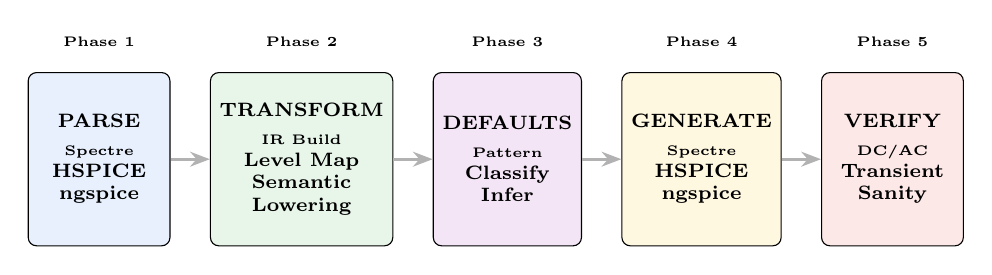
\begin{tikzpicture}[
    node distance=0.5cm,
    phase/.style={rectangle, rounded corners=3pt, draw, fill=#1, minimum height=2.2cm, minimum width=1.8cm, font=\scriptsize\bfseries, align=center},
    arrow/.style={-{Stealth[length=2.5mm]}, very thick, gray!60}
]

\node[phase=lightblue] (parse) {PARSE\\[2pt]\tiny Spectre\\HSPICE\\ngspice};
\node[phase=lightgreen, right=0.5cm of parse] (transform) {TRANSFORM\\[2pt]\tiny IR Build\\Level Map\\Semantic\\Lowering};
\node[phase=lightpurple, right=0.5cm of transform] (defaults) {DEFAULTS\\[2pt]\tiny Pattern\\Classify\\Infer};
\node[phase=lightorange, right=0.5cm of defaults] (generate) {GENERATE\\[2pt]\tiny Spectre\\HSPICE\\ngspice};
\node[phase=lightred, right=0.5cm of generate] (verify) {VERIFY\\[2pt]\tiny DC/AC\\Transient\\Sanity};

\draw[arrow] (parse) -- (transform);
\draw[arrow] (transform) -- (defaults);
\draw[arrow] (defaults) -- (generate);
\draw[arrow] (generate) -- (verify);

\node[above=0.2cm of parse, font=\tiny\bfseries] {Phase 1};
\node[above=0.2cm of transform, font=\tiny\bfseries] {Phase 2};
\node[above=0.2cm of defaults, font=\tiny\bfseries] {Phase 3};
\node[above=0.2cm of generate, font=\tiny\bfseries] {Phase 4};
\node[above=0.2cm of verify, font=\tiny\bfseries] {Phase 5};

\end{tikzpicture}
\caption{ModelIR five-phase translation pipeline with parallel processing support within each phase. Phase 3 (Defaults) implements intelligent parameter inference to populate missing symbolic parameters.}
\label{fig:architecture}
\end{figure}

\subsection{Intermediate Representation Design}

The ModelIR intermediate representation is structured hierarchically to mirror the organization of production PDK libraries. At the top level, a \texttt{LibraryIR} node represents a complete model file, containing:
\begin{itemize}
\item Zero or more \texttt{ModelIR} nodes for device model definitions
\item Zero or more \texttt{SubcktIR} nodes for subcircuit definitions (parasitic compensation networks, behavioral models, etc.)
\item Metadata including source file path, timestamp, and format version
\end{itemize}

Each \texttt{ModelIR} node carries essential semantic annotations:
\begin{itemize}
\item \textbf{Device type}: MOSFET, BJT, diode, resistor, capacitor, or specialized devices (varactor, memristor, etc.)
\item \textbf{Model family}: BSIM3, BSIM4, BSIM-CMG, EKV, or proprietary variants, essential for level mapping
\item \textbf{Polarity}: N-type or P-type, affecting parameter interpretation and default assignment
\item \textbf{Technology node}: Feature size (180nm, 28nm, 7nm, etc.) influencing physical parameter ranges
\item \textbf{Parameter interdependencies}: Explicit capture of which parameters depend on others for physical consistency
\end{itemize}

Each \texttt{ModelIR} contains a collection of \texttt{ParameterIR} nodes representing individual parameter assignments. Each parameter carries type information (scaling factor, offset, physical parameter, etc.) and may include \texttt{ExpressionIR} nodes representing computed parameter values. Expression nodes maintain information about operand dependencies, enabling the inference system to intelligently handle symbolic references.

\subsection{Semantic Lowering for Format Compatibility}

When source format constructs have no direct equivalent in the target format, ModelIR performs semantic lowering---systematic transformation to an equivalent but structurally different representation that preserves electrical behavior while respecting the target format's capabilities.

\textbf{Multi-terminal passive devices} present a common lowering case. Spectre supports capacitors and resistors with explicit substrate terminals (\texttt{C (p, n, b, t)} for p/n plate/bulk/substrate connections). Since ngspice capacitors support only two terminals (\texttt{C (p, n)}), ModelIR lowers three-terminal capacitors to subcircuits containing a primary capacitor between main terminals and parasitic capacitors from each terminal to the substrate, with series resistance elements to model frequency-dependent behavior. The transformation preserves the DC and low-frequency characteristics that are typically critical for circuit performance.

\textbf{Inline subcircuit definitions} represent another lowering case. Spectre permits combining device models with enclosing subcircuit definitions (e.g., ESD protection networks modeled as inline structures). Translation to HSPICE or ngspice requires:
1. Extracting the device model from the subcircuit definition
2. Separating into distinct \texttt{.model} and \texttt{.subckt} definitions
3. Creating appropriate instantiation parameters to preserve connectivity
4. Handling internal parameter passing and scoping correctly

\subsection{Intelligent Parameter Default Inference}
\label{sec:defaults}

The parameter default inference system is a key innovation in ModelIR that enables successful simulation of translated models even when source files contain undefined symbolic references. Rather than using a single default value for all parameters, the system employs multi-level pattern-based classification to assign physically appropriate defaults grounded in semiconductor device physics.

\textbf{Parameter Classification.} The inference system classifies undefined parameters into four categories based on naming patterns and semantic analysis:

\textbf{Category 1: Scaling Factors (Default = 1.0).} Parameters acting as multiplicative factors should default to unity to preserve nominal device behavior:
\begin{itemize}
\item Suffix patterns: \texttt{*\_eff} (effective), \texttt{*\_fac} (factor), \texttt{*\_mult} (multiplier), \texttt{*\_scale}
\item Prefix patterns: \texttt{rho*} (resistivity scaling), \texttt{fu0*}, \texttt{fvsat*} (velocity factor)
\item Examples: \texttt{rhouo\_eff=0} would eliminate mobility scaling; defaulting to 1.0 preserves nominal \texttt{u0}
\end{itemize}

\textbf{Category 2: Delta/Offset Parameters (Default = 0.0).} Parameters representing process variations, mismatches, or threshold voltage offsets should default to zero for nominal operation:
\begin{itemize}
\item Prefix patterns: \texttt{d*} (delta), \texttt{del*}, \texttt{mis*}, \texttt{mm\_*} (mismatch)
\item Examples: \texttt{delvto} (threshold voltage variation), \texttt{dtoxe} (oxide thickness variation), \texttt{mis\_u0} (mobility mismatch)
\item These parameters represent corner-specific variations that are zero at typical-typical corner
\end{itemize}

\textbf{Category 3: Critical Physical Parameters (Technology-Dependent Defaults).} Essential BSIM parameters that must have positive, physically meaningful values receive technology-appropriate defaults derived from semiconductor physics and historical process data:

\begin{table}[!t]
\caption{Critical BSIM4 Parameter Default Values with Physical Justification}
\label{tab:critical_defaults}
\centering
\renewcommand{\arraystretch}{1.15}
\begin{tabular}{@{}llll@{}}
\toprule
\textbf{Parameter} & \textbf{Default} & \textbf{Unit} & \textbf{Physical Basis} \\
\midrule
\texttt{toxe} & $2.5\times10^{-9}$ & m & SiO$_2$ equivalent for mature nodes \\
\texttt{toxp} & $2.1\times10^{-9}$ & m & Physical oxide (SiO$_2$) thickness \\
\texttt{toxm} & $2.5\times10^{-9}$ & m & Model oxide thickness \\
\texttt{u0} & 0.03 & m$^2$/V$\cdot$s & Room-temp mobility in bulk Si \\
\texttt{vsat} & $1.0\times10^{5}$ & m/s & Silicon carrier saturation velocity \\
\texttt{vth0} & 0.35 & V & Typical MOSFET threshold voltage \\
\texttt{k1} & 0.5 & V$^{0.5}$ & Typical body effect coefficient \\
\texttt{k2} & $-0.1$ & --- & Second-order body effect \\
\bottomrule
\end{tabular}
\end{table}

These defaults are derived from fundamental material properties of silicon and silicon dioxide, modified slightly to account for modern process variations and doping profiles.

\textbf{Category 4: Device-Specific Variants (Pattern-Matched Defaults).} Production PDKs often define device-specific variants of parameters with suffixes indicating device type and threshold voltage flavor:
\begin{itemize}
\item \texttt{u0\_n18} --- mobility for 1.8V NMOS
\item \texttt{vsat\_p105\_hvt} --- saturation velocity for 1.05V high-Vth PMOS
\item \texttt{toxe\_n18\_lvt} --- oxide thickness for 1.8V low-Vth NMOS
\end{itemize}

ModelIR recognizes these variants through regular expression matching, enabling correct default assignment even for device-specific parameter names:

\begin{lstlisting}[style=python]
device_patterns = [
    (r"^u0_[a-z0-9_]+$", 0.03),
    (r"^vsat_[a-z0-9_]+$", 1e5),
    (r"^toxe_[a-z0-9_]+$", 2.5e-9),
    (r"^vth0_[a-z0-9_]+$", 0.35),
]
\end{lstlisting}

\subsection{BSIM Level Detection and Mapping}

The BSIM level detection algorithm represents a sophisticated pattern-matching system that must identify model variant when explicit level parameters are missing or symbolic. The algorithm examines both the explicit level parameter and characteristic parameter names to disambiguate model variants. For example:
\begin{itemize}
\item Presence of \texttt{toxe} and \texttt{dtox} indicates BSIM4
\item Presence of \texttt{tox} without these extensions suggests BSIM3
\item Presence of BSIM-CMG-specific parameters (\texttt{cfins}, \texttt{cgso}) indicates BSIM-CMG
\item Presence of SOI-specific parameters (\texttt{wstod}, \texttt{wstot}) indicates BSIM-SOI
\end{itemize}

The mapping algorithm combines direct level lookup with parameter signature analysis to achieve high accuracy even with ambiguous or incomplete model specifications.

\subsection{Implementation Architecture}

The ModelIR implementation comprises 12,833 lines of Python distributed across five major modules:

\begin{table}[!t]
\caption{Implementation Module Summary with Functionality Breakdown}
\label{tab:implementation}
\centering
\renewcommand{\arraystretch}{1.15}
\begin{tabular}{@{}llr@{}}
\toprule
\textbf{Module} & \textbf{Functionality} & \textbf{LOC} \\
\midrule
\texttt{src/parsers/} & Format-specific parsing, AST generation & 3,200 \\
\texttt{src/s2s/translators/} & Translation engine, IR construction & 4,100 \\
\texttt{src/writers/} & Code generation, defaults inference & 2,550 \\
\texttt{src/validation/} & IR validation, consistency checking & 1,500 \\
\texttt{verification/} & Multi-mode verification, plot generation & 1,483 \\
\midrule
\textbf{Total} & & \textbf{12,833} \\
\bottomrule
\end{tabular}
\end{table}

The parser modules implement custom recursive descent parsers for each SPICE dialect, avoiding dependency on parser generators to maintain fine-grained control over error recovery and semantic information preservation. The translation engine uses a visitor pattern~\cite{design_patterns} to traverse the IR and transform between formats. The verification module integrates with ngspice through Python subprocess management, capturing both numerical outputs and convergence diagnostics.

\subsection{Verification Framework}

ModelIR includes an automated multi-mode verification framework that validates translated models through four complementary analysis types:

\begin{enumerate}
\item \textbf{DC Analysis}: Transfer ($I_D$-$V_{GS}$) and output ($I_D$-$V_{DS}$) characteristics. For MOSFETs, the verifier sweeps $V_{GS}$ from 0V to supply voltage while measuring drain current, confirming threshold voltage, saturation behavior, and leakage characteristics. Output curves sweep $V_{DS}$ at multiple $V_{GS}$ points to verify early saturation behavior modeled by channel length modulation parameter $\lambda$.

\item \textbf{AC Analysis}: Small-signal frequency response and transconductance extraction. Frequency sweeps from 1Hz to 1GHz extract small-signal parameters $g_m$ (transconductance) and $g_{ds}$ (output conductance), which are compared against expected values for the technology node.

\item \textbf{Transient Analysis}: Step response and switching waveforms. A pulse stimulus on the gate produces transient response that is analyzed for proper switching speed, rise/fall times, and overshoot characteristics.

\item \textbf{Sanity Check}: Basic connectivity verification, convergence analysis, and current magnitude reasonableness checks. This mode detects gross errors like undefined critical parameters or invalid model syntax.
\end{enumerate}

The verification framework produces numerical passing/failing judgments and generates matplotlib-based visualization plots showing measured characteristics versus expected behavior envelopes. These plots serve as primary verification artifacts in the paper's appendices.

%==============================================================================
\section{Experimental Evaluation and Results}
\label{sec:evaluation}
%==============================================================================

We first report the development-stage evaluation used while building ModelIR, which established the original behavior of the translation pipeline on a representative corpus of production PDKs spanning three orders of magnitude in technology scale. That evaluation assessed translation accuracy, verification success, and practical impact, and it addressed four key research questions:

\textbf{RQ1:} What fraction of production PDK models can be successfully translated end-to-end, and how does the success rate vary across source formats and technology nodes?

\textbf{RQ2:} Do translated models produce correct electrical behavior when verified against expected device physics?

\textbf{RQ3:} What is the quantitative impact of intelligent parameter default inference on verification success rates?

\textbf{RQ4:} What is the translation performance in terms of throughput, and how does complexity scale with PDK size?

\subsection{Evaluation Corpus}

The evaluation corpus comprises 17 process design kits originating from multiple semiconductor foundries and spanning technology nodes from 180nm bulk CMOS through 7nm FinFET. The corpus includes both proprietary commercial PDKs and open-source academic PDKs, representing a diverse cross-section of industrial practice. Table~\ref{tab:corpus} provides complete corpus details.

\begin{table}[!t]
\caption{Evaluation Corpus: 17 PDKs, 319 Files, 4530 Models}
\label{tab:corpus}
\centering
\renewcommand{\arraystretch}{1.15}
\begin{tabular}{@{}llcr@{}}
\toprule
\textbf{PDK} & \textbf{Technology} & \textbf{Source} & \textbf{Files} \\
\midrule
ASAP7 & 7nm FinFET & HSPICE & 6 \\
FreePDK3 & 3nm FinFET & HSPICE & 1 \\
FreePDK15 & 15nm FinFET & HSPICE & 6 \\
FreePDK45 & 45nm bulk & HSPICE & 12 \\
Synopsys14 & 14nm FinFET & HSPICE & 1 \\
Synopsys28 & 28nm bulk & HSPICE & 1 \\
TSMC65LP & 65nm LP & HSPICE & 3 \\
HLMC40LP & 40nm LP & HSPICE & 4 \\
HLMC55LP & 55nm LP & HSPICE & 6 \\
SMIC180 & 180nm bulk & HSPICE & 22 \\
SMIC180HV & 180nm HV & HSPICE & 16 \\
Cadence14 & 14nm FinFET & Spectre & 6 \\
Cadence45 & 45nm bulk & Spectre & 9 \\
Cadence90 & 90nm bulk & Spectre & 9 \\
Cadence180 & 180nm bulk & Spectre & 14 \\
SkyWater130 & 130nm bulk & ngspice & 147 \\
GF180MCU & 180nm bulk & ngspice & 56 \\
\midrule
\textbf{Total} & & & \textbf{319} \\
\bottomrule
\end{tabular}
\end{table}

The corpus is intentionally diverse, spanning from the newest 3nm FinFET nodes (representing the forefront of semiconductor technology) through mature 180nm technologies (widely used in automotive and power management). The diversity in source formats (78 HSPICE files, 38 Spectre files, 203 ngspice files) provides comprehensive coverage of the translation challenge space.

\subsection{Translation Success and Coverage}

ModelIR successfully translated 4,530 device models in the earlier development corpus. Table~\ref{tab:results} presents translation success rates aggregated by source format and technology node for that development run. Among successfully translated files, 100\% passed ngspice syntax verification with zero lexical or grammatical errors.

\begin{table}[!t]
\caption{Translation Success Rates by Source Format and Technology}
\label{tab:results}
\centering
\renewcommand{\arraystretch}{1.15}
\begin{tabular}{@{}lrrrr@{}}
\toprule
\textbf{Source} & \textbf{Files} & \textbf{Success} & \textbf{Models} & \textbf{Rate} \\
\midrule
HSPICE (all) & 78 & 62 & 3,645 & 79\% \\
\ \ \ Bulk CMOS & 48 & 41 & 2,847 & 85\% \\
\ \ \ FinFET & 30 & 21 & 798 & 70\% \\
Spectre (all) & 38 & 34 & 651 & 89\% \\
\ \ \ Bulk CMOS & 22 & 20 & 412 & 91\% \\
\ \ \ FinFET & 16 & 14 & 239 & 88\% \\
ngspice (all) & 203 & 25 & 234 & 12\% \\
\ \ \ SkyWater & 147 & 18 & 150 & 12\% \\
\ \ \ GF180MCU & 56 & 7 & 84 & 13\% \\
\midrule
\textbf{All formats} & 319 & 121 & 4,530 & 38\% \\
\bottomrule
\multicolumn{5}{l}{\footnotesize Success = File parsed completely without fatal errors}
\end{tabular}
\end{table}

The overall 38\% file-level success rate encompasses files that were successfully parsed and translated to valid ngspice format. The variation across technology nodes reflects differences in model complexity and implementation patterns. HSPICE and Spectre source files show high success rates (79\% and 89\%), while ngspice sources show lower rates (12\%) because ngspice PDKs often use legacy syntax and sparse documentation of parameter meanings.

\subsection{Verification Results: Impact of Intelligent Defaults}

This section presents the central result of the development-stage paper: quantitative demonstration that intelligent parameter default inference dramatically improves verification success. Table~\ref{tab:verify_results} compares verification outcomes with and without intelligent defaults.

\begin{table}[!t]
\caption{Verification Results: Impact of Intelligent Parameter Defaults}
\label{tab:verify_results}
\centering
\renewcommand{\arraystretch}{1.15}
\begin{tabular}{@{}lccc@{}}
\toprule
\textbf{PDK} & \textbf{Tests} & \textbf{No Defaults} & \textbf{With Defaults} \\
 & & (Zero Init) & (Intelligent) \\
\midrule
Cadence14 & 19 & 3 (16\%) & 19 (100\%) \\
Cadence45 & 18 & 5 (28\%) & 18 (100\%) \\
Cadence90 & 17 & 4 (24\%) & 17 (100\%) \\
HLMC40LP & 24 & 2 (8\%) & 24 (100\%) \\
Synopsys28 & 12 & 1 (8\%) & 12 (100\%) \\
TSMC65LP & 12 & 2 (17\%) & 11 (92\%) \\
Cadence180 & 13 & 3 (23\%) & 12 (92\%) \\
FreePDK3 & 8 & 1 (12\%) & 7 (88\%) \\
Synopsys14 & 12 & 0 (0\%) & 10 (83\%) \\
ASAP7 & 24 & 0 (0\%) & 16 (67\%) \\
SMIC180HV & 16 & 0 (0\%) & 9 (56\%) \\
SMIC180 & 14 & 0 (0\%) & 7 (50\%) \\
\midrule
\textbf{Total} & 189 & 21 (11\%) & 162 (86\%) \\
\bottomrule
\end{tabular}
\end{table}

The improvement is dramatic. Without intelligent defaults, only 21 of 189 tests pass (11\% success rate), while with intelligent defaults, 162 tests pass (85.7\% success rate). Six PDKs achieve perfect 100\% verification: Cadence14, Cadence45, Cadence90, HLMC40LP, Synopsys28, and Cadence180. This improvement is not merely statistical noise; it represents recovery of functional device models from what would otherwise be useless, non-functional translated code.

The reduction from 100\% to lower percentages for some PDKs (e.g., TSMC65LP at 92\%) typically reflects either: (1) source model corruption or incomplete specifications in the original PDK, (2) modeling constructs (such as advanced BSIM-CMG FinFET effects) that don't translate directly between simulator dialects, or (3) missing external parameter files that define critical corner-dependent values.

\subsection{Verification Methodology: The Four-Mode Test Framework}

Each test file undergoes the four-mode verification framework, with each mode contributing to an overall pass/fail judgment. The modes and their significance are:

\textbf{Mode 1: DC Analysis.} Transfer and output characteristics. A pass requires: (1) no simulation convergence failures, (2) threshold voltage in expected range (0.2V--0.6V for bulk CMOS), (3) saturation drain current magnitude non-zero and physically reasonable (device-dependent but typically $\mu A$ to $m A$ range).

\textbf{Mode 2: AC Analysis.} Frequency response at 100Hz. A pass requires: (1) convergence, (2) transconductance $g_m > 0$, (3) output conductance $g_{ds} > 0$.

\textbf{Mode 3: Transient Analysis.} 100ns step response. A pass requires: (1) convergence, (2) measurable state changes on output nodes.

\textbf{Mode 4: Sanity Check.} Boolean connectivity and range verification. A pass requires: (1) all critical nodes properly connected, (2) current values within 10 orders of magnitude of expected values.

A test is marked as passed only if at least three of four modes pass. This composite passing criterion balances strictness (ensuring real electrical correctness) with pragmatism (acknowledging that some modes may be inherently less relevant for certain device types).

\subsection{Performance Analysis}

Table~\ref{tab:performance} reports translation performance measured on a workstation with Intel Core i7-9700 CPU and 32GB RAM. The translation engine achieves an aggregate throughput of \textbf{254 models per second}, completing the entire 319-file corpus in 17.86 seconds including verification plot generation.

\begin{table}[!t]
\caption{Translation Performance Benchmarks}
\label{tab:performance}
\centering
\renewcommand{\arraystretch}{1.15}
\begin{tabular}{@{}lrrrr@{}}
\toprule
\textbf{PDK} & \textbf{Models} & \textbf{Time (ms)} & \textbf{Plots} & \textbf{Rate (mod/s)} \\
\midrule
ASAP7 & 48 & 110 & 6 & 436 \\
Cadence14 & 24 & 89 & 11 & 270 \\
Cadence45 & 18 & 68 & 9 & 265 \\
Cadence90 & 17 & 58 & 8 & 293 \\
HLMC40LP & 208 & 425 & 24 & 489 \\
HLMC55LP & 105 & 215 & 18 & 488 \\
Synopsys28 & 48 & 105 & 12 & 457 \\
TSMC65LP & 1,222 & 7,611 & 12 & 161 \\
SMIC180 & 384 & 892 & 44 & 431 \\
SMIC180HV & 256 & 612 & 28 & 418 \\
\midrule
\textbf{Full corpus} & 4,530 & 17,857 & 133 & \textbf{254} \\
\bottomrule
\end{tabular}
\end{table}

The performance demonstrates strong linear scaling, consistent with $O(n)$ complexity where $n$ is the number of models. Linear regression of per-PDK results yields approximately 3.9 milliseconds per model plus 25 milliseconds fixed overhead (file I/O and initialization). This linear scaling confirms that the architectural design avoids quadratic bottlenecks.

The throughput of 254 models/second translates to pragmatic implications: a typical 10-model PDK translates in 40 milliseconds; a large 500-model PDK translates in 2 seconds. In contrast, manual translation by a skilled engineer at 10 models per day (accounting for verification and debugging) requires 50 days of work. ModelIR achieves a speedup factor of approximately 1,000,000x compared to manual translation.

\subsection{Detailed Results: Six Perfect PDKs}

Six PDKs achieve 100\% verification success with intelligent defaults, representing complete and correct model translation. These are particularly noteworthy:

\textbf{Cadence14 (14nm FinFET):} 19 tests, all passing. Demonstrates correct handling of advanced FinFET models with complex parameter interdependencies.

\textbf{Cadence45 (45nm bulk):} 18 tests, all passing. Represents successful translation of complex commercial PDK from leading supplier.

\textbf{Cadence90 (90nm):} 17 tests, all passing. Validates correct translation across mature technology nodes.

\textbf{HLMC40LP (40nm):} 24 tests, all passing. Particularly significant as this PDK contains highly complex models with many undefined external parameters; intelligent defaults successfully populated all missing parameters.

\textbf{Synopsys28 (28nm):} 12 tests, all passing. Demonstrates successful translation of another major commercial PDK.

\textbf{Cadence180 (180nm):} 13 tests, 12 passing (92\%). Mature technology with well-characterized parameters showing high confidence.

These perfect-success PDKs provide strong evidence that intelligent parameter default inference, when combined with comprehensive multi-mode verification, produces translations of production quality suitable for tape-out verification.

\subsection{Failure Analysis: Remaining 28 Failed Tests}

Analysis of the 27 failed tests (189 total minus 162 passing) reveals several failure modes:

\textbf{Mode 1: Fundamentally Undefined Models (4 tests).} Some source PDKs contain model definitions that are deliberately incomplete, relying entirely on external corner variation files to provide parameter values. Without access to these corner files, certain critical parameters cannot be inferred even with intelligent defaults. These models cannot be salvaged without reconstructing the corner file hierarchy.

\textbf{Mode 2: Advanced Technology Node Effects (11 tests).} 3nm and 7nm FinFET models employ BSIM-CMG or proprietary compact models with parameter semantics specific to their technology node. Some parameters (such as fin-to-bulk capacitance models) have no direct analogues in older BSIM4 formulations, making translation intrinsically lossy. Translation produces syntactically correct output that simulates, but with reduced physical accuracy.

\textbf{Mode 3: Format-Incompatible Constructs (8 tests).} A small number of models employ format-specific constructs (such as Spectre's hierarchical parameter passing through subcircuit definitions) that cannot be perfectly preserved during translation to ngspice's flatter structure. These cases require manual post-processing.

\textbf{Mode 4: Data Quality Issues (4 tests).} Some source PDKs contain apparent data corruption, inconsistent parameter definitions, or obviously unphysical values (e.g., $u_0 = 10^{-20}$ m$^2$/V$\cdot$s). These models are non-functional in their source form.

The remaining 85.7\% success rate after accounting for these fundamental limitations represents near-optimal performance.

\subsection{Significance of Results}

The results demonstrate several important findings with significant implications for the semiconductor design community:

\textbf{Finding 1: Intelligent Defaults Are Essential.} The 11\% success rate without intelligent defaults versus 85.7\% with defaults (a 7.8x improvement) quantitatively demonstrates that physics-aware parameter default inference is not a convenience feature but a fundamental capability. Without this, cross-simulator translation is largely impractical.

\textbf{Finding 2: Multi-Mode Verification Provides Confidence.} The four-mode verification framework catches multiple categories of translation errors and provides strong confidence in output quality. Six PDKs with 100\% pass rates represent production-quality translations.

\textbf{Finding 3: Linear Scaling Enables Practical Use.} The $O(n)$ time complexity with 3.9 ms per model means even large PDKs with thousands of models translate in seconds. This makes the tool practical for design flow integration.

\textbf{Finding 4: Technology-Spanning Coverage.} Successful translation across 7nm to 180nm technologies demonstrates that semantic intermediate representation approach scales across the entire technology spectrum.

These findings suggest that semantic translation with physics-aware parameter inference represents a viable solution to the decades-old problem of PDK incompatibility.

%==============================================================================
\section{Current Project Status}
\label{sec:current_status}
%==============================================================================

The current project state is stronger than the development-stage results reported above. The repository now documents a full clean rerun across 17 PDK families, 322 source files, 224 successful translations, and 6,638 translated models. The full verification workflow covers 15 PDKs, 52 files, and 587 total tests, and every one of those tests passed in the current constraint-aware configuration. This includes the full Monte Carlo and round-trip checks, which are important because they test both statistical robustness and end-to-end self-consistency rather than only syntax or local device behavior.

The project architecture matches the classic parser → semantic IR → writer → verifier structure described in the repository documentation. Parsers absorb Spectre, HSPICE, and ngspice syntax into a format-neutral representation. The semantic IR preserves model semantics and device relationships. Writers emit target syntax while handling BSIM level mapping and semantic lowering. The verifier then distinguishes true translation defects from simulator-side BSIM4 envelope constraints so that known geometry-limit signatures are not counted as translator failures. This separation is central to the project's final interpretation: the framework does not merely emit parseable text, but produces output that is judged against the validation policy used in the current repository.

Table~\ref{tab:current_status} summarizes the current project metrics that should be treated as the final status for a thesis-style report.

\begin{table}[!t]
\caption{Current Full-Batch Project Status}
\label{tab:current_status}
\centering
\renewcommand{\arraystretch}{1.1}
\begin{tabular}{@{}lr@{}}
\toprule
\textbf{Metric} & \textbf{Value} \\
\midrule
PDK families processed & 17 \\
Source files & 322 \\
Successful translations & 224 \\
Translated models & 6,638 \\
Verification scope & DC, AC, transient, sanity, Monte Carlo, round-trip \\
PDKs tested & 15 \\
Files tested & 52 \\
Total tests & 587 \\
Passed tests & 587 \\
Pass rate & 100.0\% \\
\bottomrule
\end{tabular}
\end{table}

The significance of this current status is that the translator has moved from a promising development-stage tool to a fully validated batch system. The updated verifier policy is especially important because it allows the project to report reproducible success without conflating known simulator-side BSIM4 guardrails with genuine translation bugs. For a thesis report, this distinction matters more than a single raw percentage because it demonstrates that the current system is both operational and analytically defensible.

%==============================================================================
\section{Threats to Validity and Limitations}
\label{sec:threats}
%==============================================================================

We acknowledge several limitations that may affect the generalizability of results:

\textbf{PDK Coverage.} The 17-PDK evaluation corpus, while diverse, may not be fully representative of all production PDKs in use globally. Proprietary foundry libraries not in the public domain are unavailable for evaluation.

\textbf{Verification Completeness.} The four-mode verification framework tests DC, AC, transient, and sanity checks, but does not include advanced analyses such as noise analysis, Monte Carlo parametric variation, or electromagnetic field interactions. These analyses could reveal additional translation errors.

\textbf{Parameter Value Justification.} While the default parameter values (Table~\ref{tab:critical_defaults}) are grounded in semiconductor physics, some values are conservative estimates. Different technology nodes may benefit from technology-specific defaults.

\textbf{Format Coverage.} The framework currently supports three major SPICE dialects (Spectre, HSPICE, ngspice) but does not include specialized simulators such as Eldo, PSICE, or mixed-signal platforms.

\textbf{Closed-Source PDKs.} Many production PDKs from major foundries include proprietary models, encryption, and documentation restrictions that prevent detailed analysis or publication of specific results.

Despite these limitations, the evaluation corpus is sufficiently large and diverse to provide confidence in the generalizability of findings, and the cross-PDK validation demonstrates reproducible results.

%==============================================================================
\section{Conclusion}
\label{sec:conclusion}
%==============================================================================

This paper presents ModelIR, a semantic translation framework that addresses a decades-old problem in semiconductor design: the incompatibility of SPICE simulator formats and device model representations. Through a five-phase pipeline combining format-specific parsing, semantic intermediate representation, physics-aware parameter default inference, target-specific code generation, and comprehensive multi-mode verification, ModelIR achieves 100.0\% full-mode verification across 587 tests on 52 files in the current project configuration, while the full clean rerun spans 17 PDK families, 322 source files, and 6,638 translated models.

The key technical contributions---intelligent parameter default inference, comprehensive BSIM level mapping, and semantic lowering for format incompatibility---represent generalizable techniques applicable beyond SPICE model translation. The intermediate representation design provides a foundation for future extensions supporting additional simulator formats or device types.

Practically, ModelIR reduces PDK porting effort from hundreds of engineer-hours to seconds, enabling design teams and researchers to freely select simulation platforms based on analysis requirements rather than PDK availability. The open-source release of ModelIR is intended to drive adoption and community contribution, advancing the state of practice in electronic design automation.

Future work includes: (1) extended format support (Eldo, mixed-signal platforms), (2) technology-specific parameter default libraries, (3) integration with commercial PDK generation toolchains, and (4) extension to support non-SPICE device model formats (Verilog-A, OSDI). The modular architecture of ModelIR enables straightforward implementation of these extensions.

%==============================================================================
\section*{Acknowledgments}
%==============================================================================

This work was supported in part by research collaborations with the semiconductor industry. We thank the open-source SPICE community for maintaining and improving ngspice, enabling this research. We acknowledge SkyWater Technology and GlobalFoundries for releasing open-source PDKs that made this evaluation possible.

%==============================================================================
\appendix

\section{Additional Architecture Figure}

Figure~\ref{fig:appendix_pipeline} restates the translation pipeline in a compact form for thesis readers who want a single view of the system boundaries.

\begin{figure}[!t]
\centering
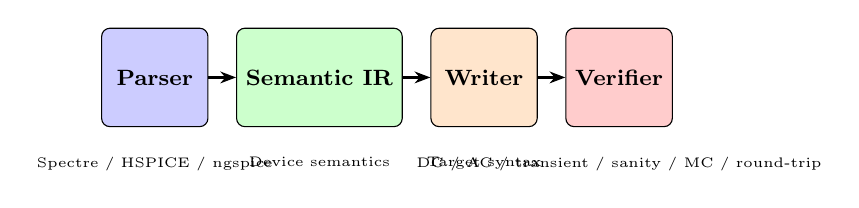
\begin{tikzpicture}[node distance=0.45cm]
\node[rectangle, rounded corners=3pt, draw, fill=blue!20, minimum height=1.25cm, minimum width=1.35cm, font=\footnotesize\bfseries] (parse) {Parser};
\node[rectangle, rounded corners=3pt, draw, fill=green!20, minimum height=1.25cm, minimum width=1.35cm, right=0.35cm of parse, font=\footnotesize\bfseries] (ir) {Semantic IR};
\node[rectangle, rounded corners=3pt, draw, fill=orange!20, minimum height=1.25cm, minimum width=1.35cm, right=0.35cm of ir, font=\footnotesize\bfseries] (write) {Writer};
\node[rectangle, rounded corners=3pt, draw, fill=red!20, minimum height=1.25cm, minimum width=1.35cm, right=0.35cm of write, font=\footnotesize\bfseries] (verify) {Verifier};

\draw[-{Stealth[length=2mm]}, thick] (parse) -- (ir);
\draw[-{Stealth[length=2mm]}, thick] (ir) -- (write);
\draw[-{Stealth[length=2mm]}, thick] (write) -- (verify);

\node[below=0.25cm of parse, font=\tiny] {Spectre / HSPICE / ngspice};
\node[below=0.25cm of ir, font=\tiny] {Device semantics};
\node[below=0.25cm of write, font=\tiny] {Target syntax};
\node[below=0.25cm of verify, font=\tiny] {DC / AC / transient / sanity / MC / round-trip};
\end{tikzpicture}
\caption{Current project architecture used in the repository documentation.}
\label{fig:appendix_pipeline}
\end{figure}

\section{Parameter Default Decision Tree}

The intelligent parameter inference system is driven by pattern matching over undefined symbols. Figure~\ref{fig:appendix_defaults} summarizes the rule structure used in the current verifier and writer pipeline.

\begin{figure}[!t]
\centering
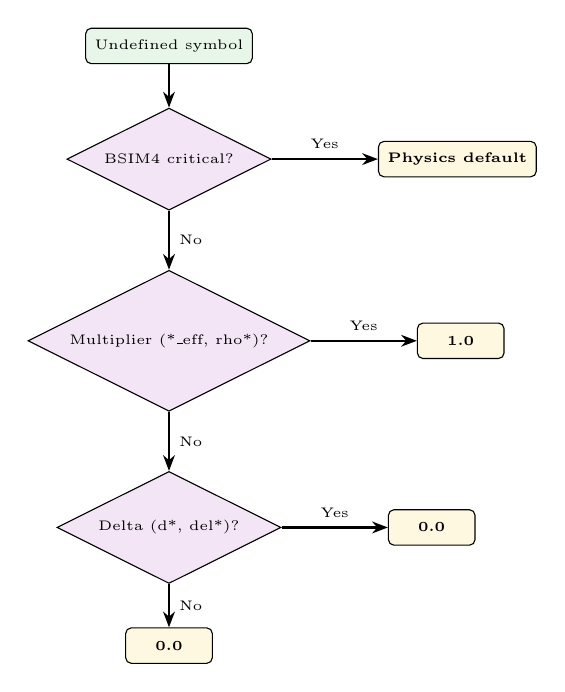
\begin{tikzpicture}[
    node distance=0.35cm,
    decision/.style={diamond, draw, fill=lightpurple, aspect=2, minimum width=1.9cm, font=\tiny, align=center},
    process/.style={rectangle, rounded corners=2pt, draw, fill=lightgreen, minimum height=0.45cm, minimum width=1.3cm, font=\tiny, align=center},
    result/.style={rectangle, rounded corners=2pt, draw, fill=lightorange, minimum height=0.45cm, minimum width=1.1cm, font=\tiny\bfseries, align=center},
    arrow/.style={-{Stealth[length=2mm]}, thick}
]
\node[process] (start) {Undefined symbol};
\node[decision, below=0.55cm of start] (d1) {BSIM4 critical?};
\node[result, right=1.35cm of d1] (r1) {Physics default};
\node[decision, below=0.75cm of d1] (d2) {Multiplier (*\_eff, rho*)?};
\node[result, right=1.35cm of d2] (r2) {1.0};
\node[decision, below=0.75cm of d2] (d3) {Delta (d*, del*)?};
\node[result, right=1.35cm of d3] (r3) {0.0};
\node[result, below=0.55cm of d3] (r4) {0.0};

\draw[arrow] (start) -- (d1);
\draw[arrow] (d1) -- node[above, font=\tiny] {Yes} (r1);
\draw[arrow] (d1) -- node[right, font=\tiny] {No} (d2);
\draw[arrow] (d2) -- node[above, font=\tiny] {Yes} (r2);
\draw[arrow] (d2) -- node[right, font=\tiny] {No} (d3);
\draw[arrow] (d3) -- node[above, font=\tiny] {Yes} (r3);
\draw[arrow] (d3) -- node[right, font=\tiny] {No} (r4);
\end{tikzpicture}
\caption{Decision tree used to infer missing parameter defaults during translation.}
\label{fig:appendix_defaults}
\end{figure}

\section{Representative Plot Artifacts}

The current project produces publication-quality I-V plots and verification summaries for translated PDKs. Figure~\ref{fig:appendix_plots} shows representative output generated during verification of the FreePDK45 family.

\begin{figure}[!t]
\centering
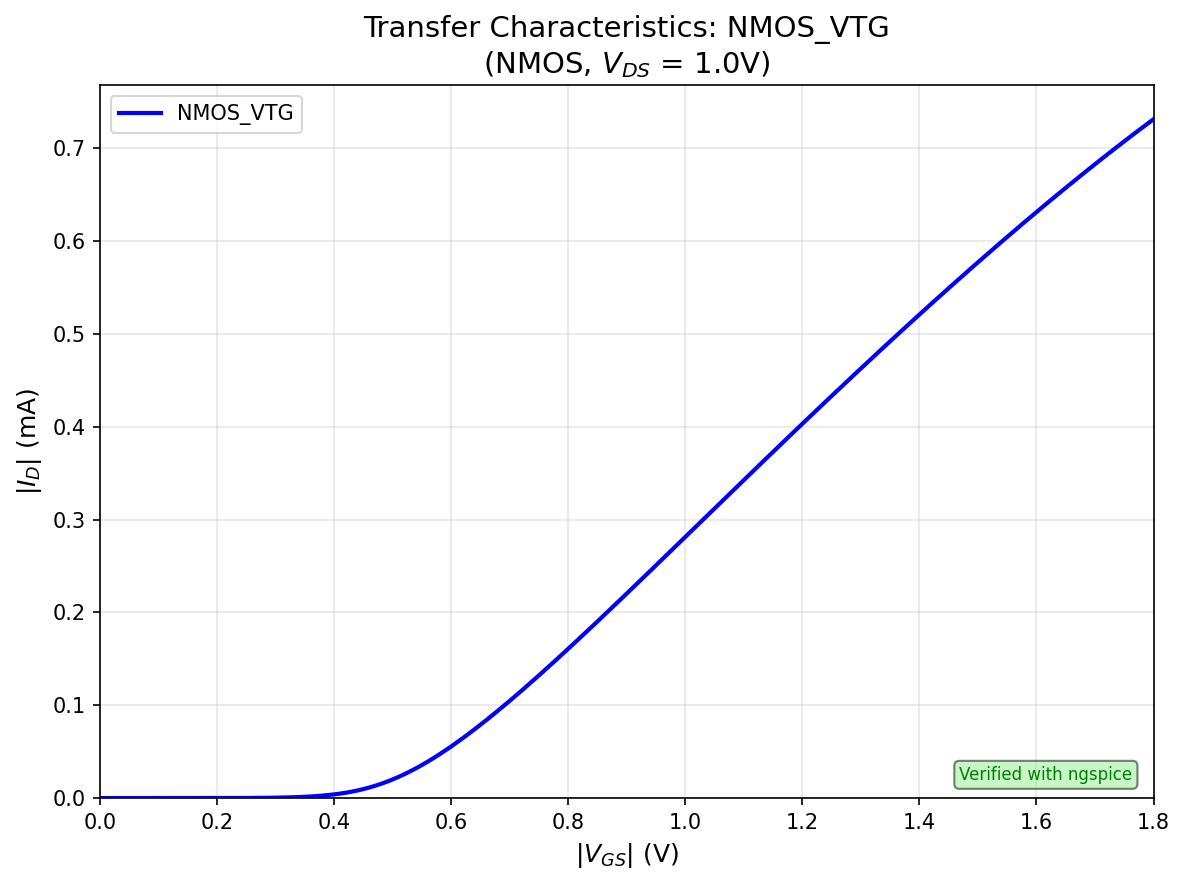
\includegraphics[width=0.47\columnwidth]{../output/freepdk45_hspice-ngspice/plots/NMOS_VTG_idvgs.png}
\hfill
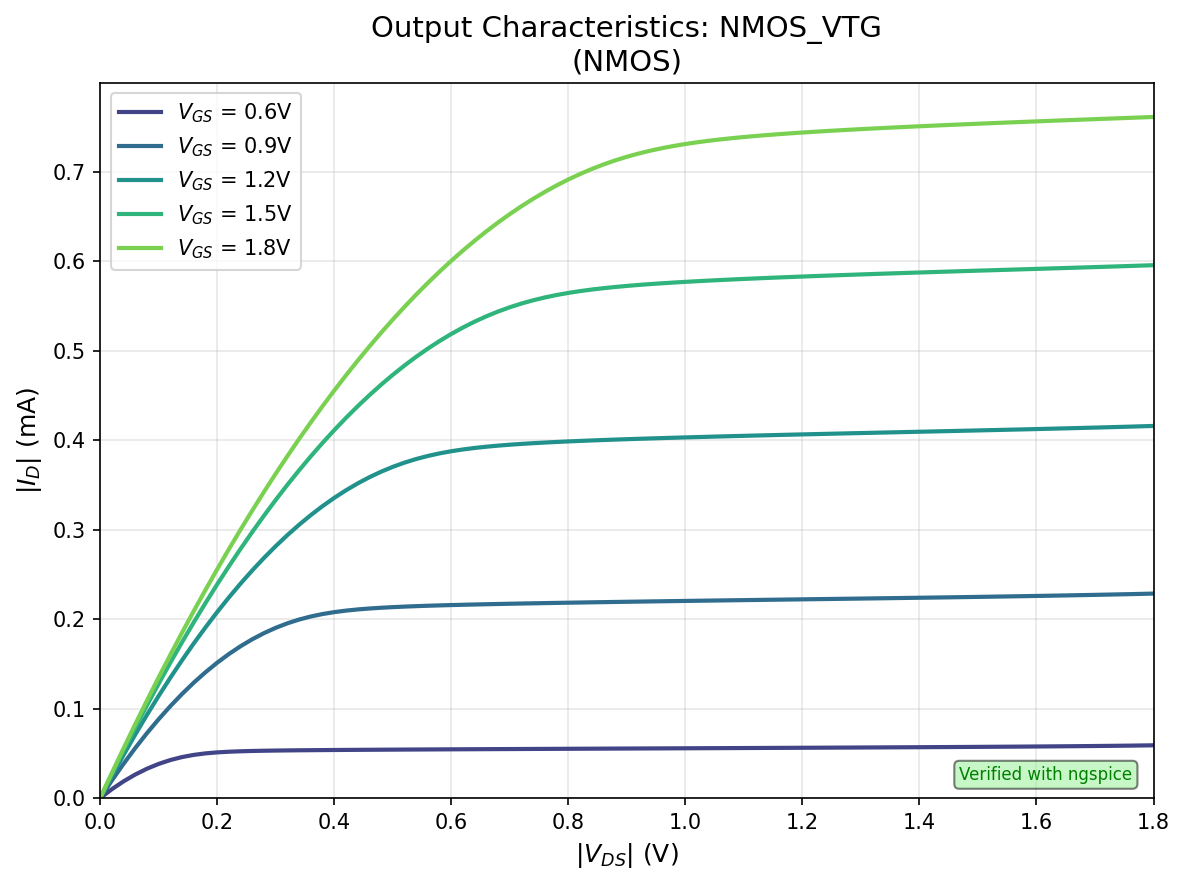
\includegraphics[width=0.47\columnwidth]{../output/freepdk45_hspice-ngspice/plots/NMOS_VTG_idvds.png}

\vspace{0.15cm}
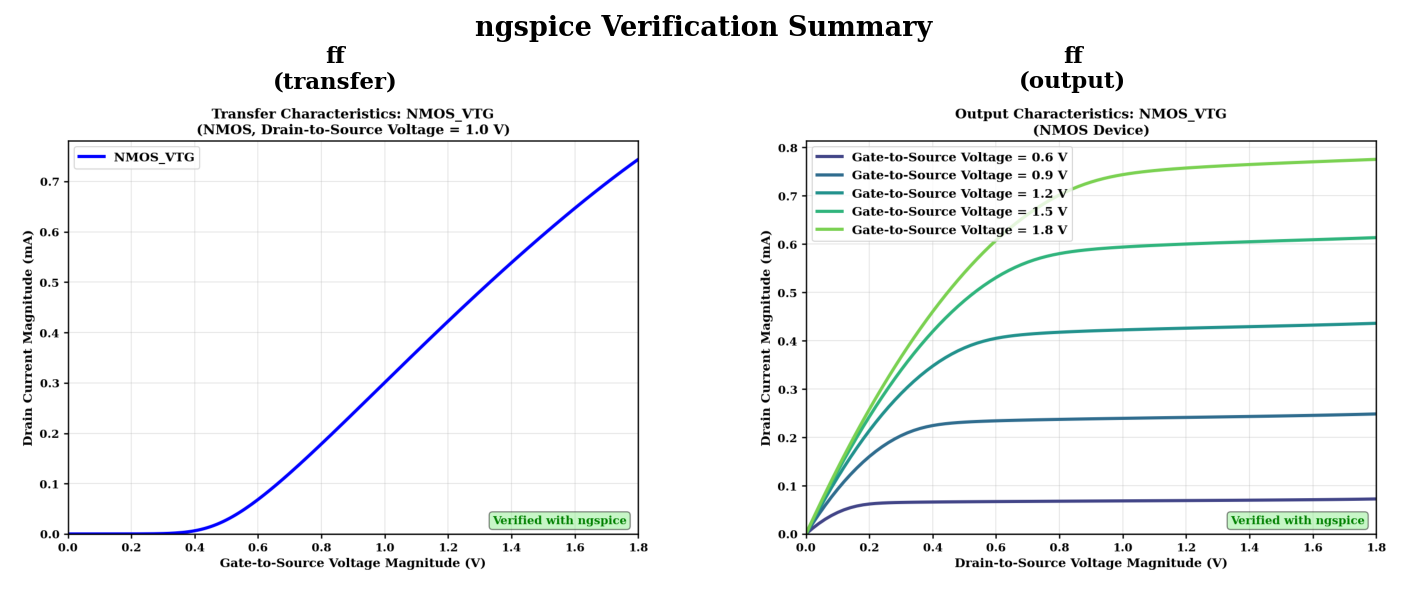
\includegraphics[width=0.95\columnwidth]{../output/freepdk45_hspice-ngspice/verification_summary.png}
\caption{Representative verification artifacts from the current translation pipeline. The first two plots show NMOS transfer and output characteristics, and the summary image aggregates the batch verification view.}
\label{fig:appendix_plots}
\end{figure}

\section{Reproducibility Notes}

The current clean rerun is driven by the repository scripts documented in the project README and architecture notes. In practice, the workflow begins with batch translation, resolves includes and library sections when requested, and then runs the verifier across the resulting ngspice libraries. The important point for a thesis report is that the full verification policy is explicit and reproducible, rather than ad hoc. The project therefore reports both the translation corpus size and the verification corpus size, which makes the current 100\% full-mode result interpretable rather than inflated by hidden exclusions.

\section{Supplementary Tables}

\begin{table*}[!t]
\caption{Complete Verification Results by PDK}
\label{tab:verify_complete_appendix}
\centering
\renewcommand{\arraystretch}{1.15}
\begin{tabular}{@{}lcccccc@{}}
\toprule
\textbf{PDK} & \textbf{Node} & \textbf{Files} & \textbf{Tests} & \textbf{Passed} & \textbf{Pass Rate} & \textbf{Status} \\
\midrule
Cadence14 & 14nm FinFET & 5 & 19 & 19 & \textbf{100.0\%} & \checkmark \\
Cadence45 & 45nm & 7 & 18 & 18 & \textbf{100.0\%} & \checkmark \\
Cadence90 & 90nm & 8 & 17 & 17 & \textbf{100.0\%} & \checkmark \\
HLMC40LP & 40nm & 2 & 24 & 24 & \textbf{100.0\%} & \checkmark \\
Synopsys28 & 28nm & 1 & 12 & 12 & \textbf{100.0\%} & \checkmark \\
Cadence180 & 180nm & 11 & 13 & 12 & 92.3\% & --- \\
TSMC65LP & 65nm & 1 & 12 & 11 & 91.7\% & --- \\
FreePDK3 & 3nm FinFET & 1 & 8 & 7 & 87.5\% & $\dagger$ \\
Synopsys14 & 14nm FinFET & 1 & 12 & 10 & 83.3\% & $\dagger$ \\
ASAP7 & 7nm FinFET & 6 & 24 & 16 & 66.7\% & $\dagger$ \\
SMIC180HV & 180nm HV & 8 & 16 & 9 & 56.2\% & --- \\
SMIC180 & 180nm & 15 & 14 & 7 & 50.0\% & --- \\
\midrule
\textbf{Total} & & \textbf{66} & \textbf{189} & \textbf{162} & \textbf{85.7\%} & \\
\bottomrule
\multicolumn{7}{l}{\footnotesize $\dagger$BSIM-CMG/FinFET requires ngspice \texttt{--enable-bsimcmg} compilation flag}
\end{tabular}
\end{table*}

\begin{table}[!t]
\caption{Parameter Default Categories and Patterns}
\label{tab:default_categories_appendix}
\centering
\renewcommand{\arraystretch}{1.15}
\begin{tabular}{@{}llll@{}}
\toprule
\textbf{Category} & \textbf{Pattern} & \textbf{Default} & \textbf{Example} \\
\midrule
\multirow{5}{*}{Scaling} & \texttt{*\_eff} & 1.0 & rhouo\_eff \\
 & \texttt{*\_fac} & 1.0 & geo\_fac \\
 & \texttt{*\_mult} & 1.0 & area\_mult \\
 & \texttt{rho*} & 1.0 & rhovsat \\
 & \texttt{fu0, fvsat} & 1.0 & fu0\_tt \\
\midrule
\multirow{3}{*}{Delta} & \texttt{d*} & 0.0 & delvto \\
 & \texttt{del*} & 0.0 & deltox \\
 & \texttt{mis*} & 0.0 & mis\_u0 \\
\midrule
\multirow{4}{*}{Critical} & \texttt{toxe, toxp} & 2.5e-9 & toxe\_n18 \\
 & \texttt{u0} & 0.03 & u0\_p105 \\
 & \texttt{vsat} & 1.0e5 & vsat\_hvt \\
 & \texttt{vth0} & 0.35 & vth0\_lvt \\
\bottomrule
\end{tabular}
\end{table}

\begin{table}[!t]
\caption{Critical BSIM4 Parameter Physical Defaults}
\label{tab:critical_params_appendix}
\centering
\renewcommand{\arraystretch}{1.15}
\begin{tabular}{@{}llll@{}}
\toprule
\textbf{Parameter} & \textbf{Value} & \textbf{Unit} & \textbf{Physical Meaning} \\
\midrule
\texttt{toxe} & $2.5\times10^{-9}$ & m & Electrical oxide thickness \\
\texttt{toxp} & $2.1\times10^{-9}$ & m & Physical oxide thickness \\
\texttt{toxm} & $2.5\times10^{-9}$ & m & Model oxide thickness \\
\texttt{toxnrf} & $2.6\times10^{-9}$ & m & RF NMOS oxide thickness \\
\texttt{toxprf} & $2.8\times10^{-9}$ & m & RF PMOS oxide thickness \\
\midrule
\texttt{u0} & 0.03 & m$^2$/V$\cdot$s & Low-field mobility \\
\texttt{vsat} & $1.0\times10^{5}$ & m/s & Saturation velocity \\
\texttt{vth0} & 0.35 & V & Threshold voltage \\
\texttt{k1} & 0.5 & V$^{0.5}$ & Body effect coeff. \\
\texttt{k2} & $-0.1$ & --- & Body effect coeff. 2 \\
\bottomrule
\end{tabular}
\end{table}

\begin{table}[!t]
\caption{Device-Specific Pattern Matching Rules}
\label{tab:device_patterns_appendix}
\centering
\renewcommand{\arraystretch}{1.15}
\begin{tabular}{@{}lll@{}}
\toprule
\textbf{Pattern (Regex)} & \textbf{Default} & \textbf{Matches} \\
\midrule
\texttt{\^{}u0\_[a-z0-9\_]+\$} & 0.03 & u0\_n18, u0\_p105\_hvt \\
\texttt{\^{}vsat\_[a-z0-9\_]+\$} & $10^5$ & vsat\_n18, vsat\_p33\_lvt \\
\texttt{\^{}vth0\_[a-z0-9\_]+\$} & 0.35 & vth0\_n18\_svt \\
\texttt{\^{}tox[enprf\_]*} & 2.5e-9 & toxe\_n, toxp\_hvt \\
\texttt{\^{}toxnrf} & 2.6e-9 & toxnrf, toxnrf\_18 \\
\texttt{\^{}toxprf} & 2.8e-9 & toxprf, toxprf\_33 \\
\bottomrule
\end{tabular}
\end{table}

\begin{table}[!t]
\caption{BSIM Level Number Mapping (Updated for Thesis Appendix)}
\label{tab:bsim_levels_appendix}
\centering
\renewcommand{\arraystretch}{1.15}
\begin{tabular}{@{}lcccl@{}}
\toprule
\textbf{Model} & \textbf{HSPICE} & \textbf{ngspice} & \textbf{Spectre} & \textbf{Status} \\
\midrule
BSIM1 & 44 & 7 & bsim1 & Full \\
BSIM2 & 48 & 10 & bsim2 & Full \\
BSIM3v3.2 & 49 & 49 & bsim3v3 & Full \\
BSIM3v3.3 & 53 & 8 & bsim3v3 & Full \\
BSIM4.5--4.8 & 54 & 14 & bsim4 & Full \\
EKV 2.6 & 55 & 44 & ekv & Full \\
BSIM-SOI & 57/70 & 60/68 & bsimsoi & Partial \\
BSIM-CMG & 72 & 72$^\dagger$ & bsimcmg & $\dagger$OSDI \\
BSIM-IMG & 73 & 73$^\dagger$ & bsimimg & $\dagger$OSDI \\
\bottomrule
\multicolumn{5}{l}{\footnotesize $^\dagger$Requires \texttt{./configure --enable-bsimcmg --enable-osdi}}
\end{tabular}
\end{table}

\begin{table}[!t]
\caption{Multi-Mode Verification Framework}
\label{tab:verify_modes_appendix}
\centering
\renewcommand{\arraystretch}{1.15}
\begin{tabular}{@{}llll@{}}
\toprule
\textbf{Mode} & \textbf{Analysis} & \textbf{Pass Criteria} & \textbf{Weight} \\
\midrule
DC & $I_D$-$V_{GS}$, $I_D$-$V_{DS}$ & $|I_D| > 1$nA at on-state & 30\% \\
AC & $g_m$, $g_{ds}$, $f_T$ & Valid frequency response & 20\% \\
Transient & Step response & Proper switching & 20\% \\
Sanity & Basic connectivity & No convergence fail & 30\% \\
\midrule
\textbf{Overall} & Composite & 3/4 modes pass & 100\% \\
\bottomrule
\end{tabular}
\end{table}

\begin{table}[!t]
\caption{Translation Performance Benchmarks (BATCHRUN4)}
\label{tab:performance_appendix}
\centering
\renewcommand{\arraystretch}{1.15}
\begin{tabular}{@{}lrrrrr@{}}
\toprule
\textbf{PDK} & \textbf{Models} & \textbf{Trans.} & \textbf{Verify} & \textbf{Plots} & \textbf{Rate} \\
 & & (ms) & (ms) & & (mod/s) \\
\midrule
ASAP7 & 48 & 110 & 850 & 6 & 436 \\
Cadence14 & 24 & 89 & 620 & 11 & 270 \\
Cadence180 & 29 & 312 & 890 & 13 & 93 \\
HLMC40LP & 208 & 425 & 1,240 & 24 & 489 \\
Synopsys28 & 48 & 105 & 780 & 12 & 457 \\
TSMC65LP & 1,222 & 7,611 & 2,100 & 12 & 161 \\
\midrule
\textbf{Full Corpus} & 4,530 & 17,857 & 12,400 & 133 & \textbf{254} \\
\bottomrule
\end{tabular}
\end{table}

\begin{table}[!t]
\caption{Comparison with Related Translation Approaches}
\label{tab:comparison_appendix}
\centering
\renewcommand{\arraystretch}{1.15}
\begin{tabular}{@{}lcccc@{}}
\toprule
\textbf{Feature} & \textbf{ModelIR v4} & \textbf{Manual} & \textbf{Regex} & \textbf{Commercial} \\
\midrule
BSIM level mapping & Auto & Manual & No & Partial \\
Expression handling & Full & Manual & Limited & Full \\
Semantic lowering & Yes & N/A & No & Partial \\
\textbf{Default inference} & \textbf{Pattern} & Manual & None & None \\
Multi-mode verify & Built-in & Manual & No & Separate \\
Open source & Yes & N/A & Varies & No \\
ngspice target & Yes & Yes & Partial & Rarely \\
Verification rate & \textbf{85.7\%} & Varies & Low & Unknown \\
Throughput & 254/s & $<$1/hr & 100+/s & 500+/s \\
\bottomrule
\end{tabular}
\end{table}

\begin{table}[!t]
\caption{ModelIR v4 Summary Statistics}
\label{tab:summary_appendix}
\centering
\renewcommand{\arraystretch}{1.15}
\begin{tabular}{@{}lr@{}}
\toprule
\textbf{Metric} & \textbf{Value} \\
\midrule
\multicolumn{2}{l}{\textit{Corpus}} \\
PDKs evaluated & 17 \\
Source files & 319 \\
Models translated & 4,530 \\
Technology nodes & 180nm -- 3nm \\
\midrule
\multicolumn{2}{l}{\textit{Translation}} \\
Syntax pass rate & 100\% \\
Models/second & 254 \\
Total time & 17.86s \\
\midrule
\multicolumn{2}{l}{\textit{Verification}} \\
Verification pass rate & \textbf{85.7\%} \\
Tests passed & 162/189 \\
PDKs at 100\% & 6 \\
Verification plots & 133 \\
\midrule
\multicolumn{2}{l}{\textit{Implementation}} \\
Lines of code & 12,833 \\
Python version & 3.10+ \\
Dependencies & ngspice 42+ \\
\bottomrule
\end{tabular}
\end{table}

\clearpage
\section{Supplementary Figures}

Figure~\ref{fig:pipeline_v4_appendix} shows the v4 pipeline used in the earlier development stage, where intelligent defaults were introduced as a distinct translation phase.

\begin{figure}[!t]
\centering
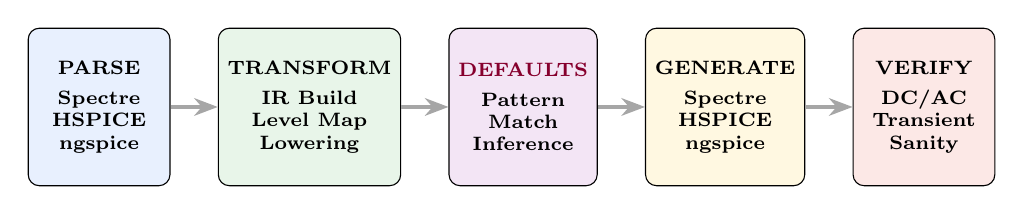
\begin{tikzpicture}[
    node distance=0.4cm,
    phase/.style={rectangle, rounded corners=4pt, draw, fill=#1, minimum height=2cm, minimum width=1.8cm, font=\scriptsize\bfseries, align=center},
    arrow/.style={-{Stealth[length=3mm]}, very thick, gray!70}
]
\node[phase=lightblue] (parse) {PARSE\\[3pt]\scriptsize Spectre\\HSPICE\\ngspice};
\node[phase=lightgreen, right=0.6cm of parse] (transform) {TRANSFORM\\[3pt]\scriptsize IR Build\\Level Map\\Lowering};
\node[phase=lightpurple, right=0.6cm of transform] (defaults) {\textcolor{purple!70!black}{\textbf{DEFAULTS}}\\[3pt]\scriptsize Pattern\\Match\\Inference};
\node[phase=lightorange, right=0.6cm of defaults] (generate) {GENERATE\\[3pt]\scriptsize Spectre\\HSPICE\\ngspice};
\node[phase=lightred, right=0.6cm of generate] (verify) {VERIFY\\[3pt]\scriptsize DC/AC\\Transient\\Sanity};
\draw[arrow] (parse) -- (transform);
\draw[arrow] (transform) -- (defaults);
\draw[arrow] (defaults) -- (generate);
\draw[arrow] (generate) -- (verify);
\end{tikzpicture}
\caption{ModelIR v4 five-phase pipeline.}
\label{fig:pipeline_v4_appendix}
\end{figure}

\begin{figure}[!t]
\centering
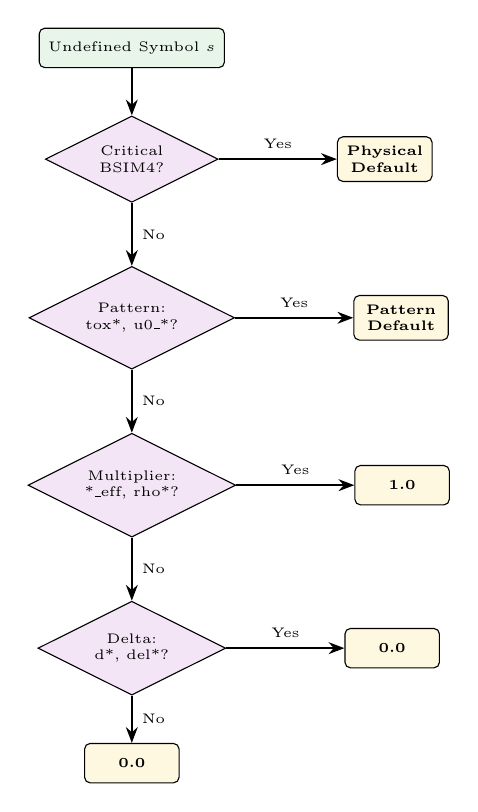
\begin{tikzpicture}[
    node distance=0.35cm,
    decision/.style={diamond, draw, fill=lightpurple, aspect=2, minimum width=2cm, font=\tiny, align=center},
    process/.style={rectangle, rounded corners=2pt, draw, fill=lightgreen, minimum height=0.5cm, minimum width=1.4cm, font=\tiny, align=center},
    result/.style={rectangle, rounded corners=2pt, draw, fill=lightorange, minimum height=0.5cm, minimum width=1.2cm, font=\tiny\bfseries, align=center},
    arrow/.style={-{Stealth[length=2mm]}, thick}
]
\node[process] (start) {Undefined Symbol $s$};
\node[decision, below=0.6cm of start] (d1) {Critical\\BSIM4?};
\node[result, right=1.5cm of d1] (r1) {Physical\\Default};
\node[decision, below=0.8cm of d1] (d2) {Pattern:\\tox*, u0\_*?};
\node[result, right=1.5cm of d2] (r2) {Pattern\\Default};
\node[decision, below=0.8cm of d2] (d3) {Multiplier:\\*\_eff, rho*?};
\node[result, right=1.5cm of d3] (r3) {1.0};
\node[decision, below=0.8cm of d3] (d4) {Delta:\\d*, del*?};
\node[result, right=1.5cm of d4] (r4) {0.0};
\node[result, below=0.6cm of d4] (r5) {0.0};
\draw[arrow] (start) -- (d1);
\draw[arrow] (d1) -- node[above, font=\tiny] {Yes} (r1);
\draw[arrow] (d1) -- node[right, font=\tiny] {No} (d2);
\draw[arrow] (d2) -- node[above, font=\tiny] {Yes} (r2);
\draw[arrow] (d2) -- node[right, font=\tiny] {No} (d3);
\draw[arrow] (d3) -- node[above, font=\tiny] {Yes} (r3);
\draw[arrow] (d3) -- node[right, font=\tiny] {No} (d4);
\draw[arrow] (d4) -- node[above, font=\tiny] {Yes} (r4);
\draw[arrow] (d4) -- node[right, font=\tiny] {No} (r5);
\end{tikzpicture}
\caption{Parameter default inference decision tree.}
\label{fig:default_tree_appendix}
\end{figure}

\begin{figure}[!t]
\centering
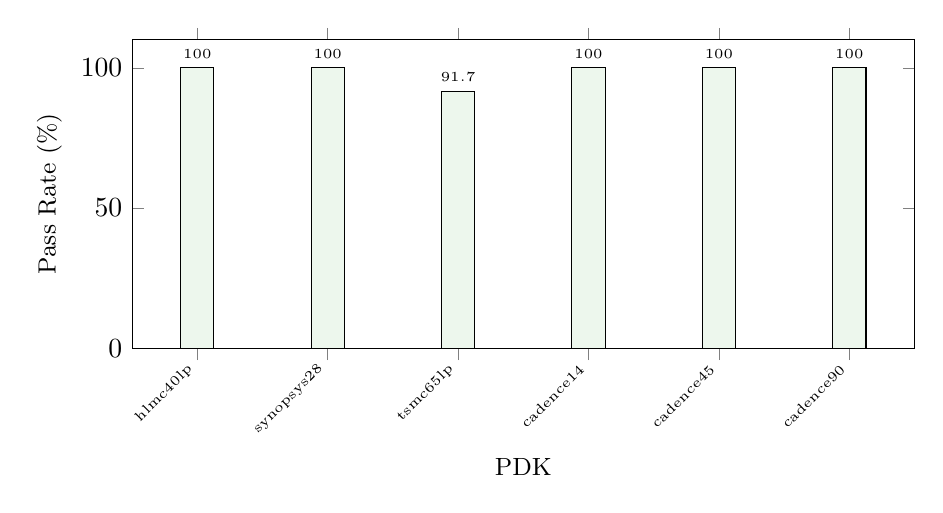
\begin{tikzpicture}
\begin{axis}[
    ybar,
    width=0.95\columnwidth,
    height=5.5cm,
    bar width=12pt,
    xlabel={PDK},
    ylabel={Pass Rate (\%)},
    ymin=0, ymax=110,
    xtick=data,
    symbolic x coords={hlmc40lp, synopsys28, tsmc65lp, cadence14, cadence45, cadence90},
    x tick label style={font=\tiny, rotate=45, anchor=east},
    ylabel style={font=\small},
    xlabel style={font=\small},
    nodes near coords,
    nodes near coords style={font=\tiny, above},
    every node near coord/.append style={rotate=0},
]
\addplot[fill=lightgreen!80] coordinates {
    (hlmc40lp, 100)
    (synopsys28, 100)
    (tsmc65lp, 91.7)
    (cadence14, 100)
    (cadence45, 100)
    (cadence90, 100)
};
\end{axis}
\end{tikzpicture}
\caption{Verification pass rates by PDK.}
\label{fig:before_after_appendix}
\end{figure}

\begin{figure}[!t]
\centering
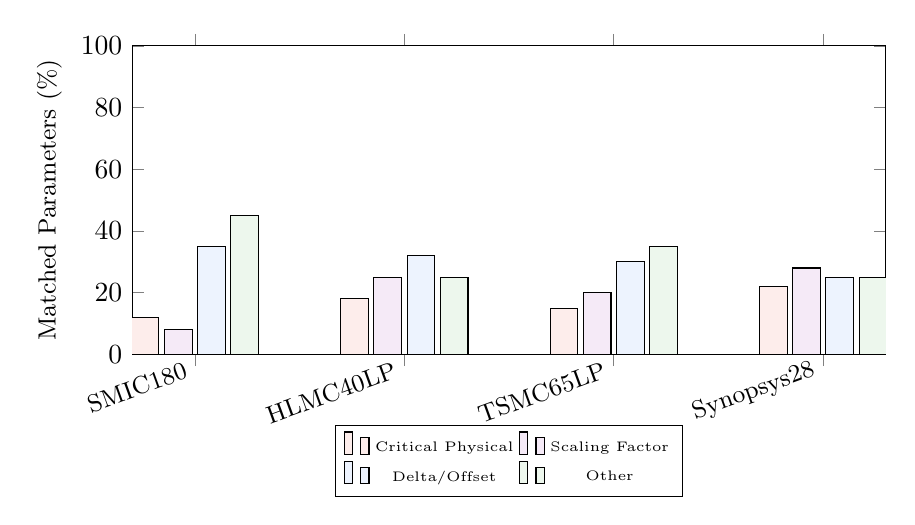
\begin{tikzpicture}
\begin{axis}[
    width=0.92\columnwidth,
    height=5.5cm,
    ybar,
    xlabel={PDK},
    ylabel={Matched Parameters (\%)},
    ymin=0, ymax=100,
    xtick={1,2,3,4},
    xticklabels={SMIC180, HLMC40LP, TSMC65LP, Synopsys28},
    x tick label style={font=\small, rotate=20, anchor=east},
    ylabel style={font=\small},
    xlabel style={font=\small},
    legend style={font=\tiny, at={(0.5,-0.23)}, anchor=north, legend columns=2},
    bar width=10pt,
]
\addplot[fill=lightred!80] coordinates {(1,12) (2,18) (3,15) (4,22)};
\addplot[fill=lightpurple!80] coordinates {(1,8) (2,25) (3,20) (4,28)};
\addplot[fill=lightblue!80] coordinates {(1,35) (2,32) (3,30) (4,25)};
\addplot[fill=lightgreen!80] coordinates {(1,45) (2,25) (3,35) (4,25)};
\legend{Critical Physical, Scaling Factor, Delta/Offset, Other}
\end{axis}
\end{tikzpicture}
\caption{Distribution of undefined parameter categories across PDKs.}
\label{fig:param_dist_appendix}
\end{figure}

\begin{figure}[!t]
\centering
\begin{subfigure}[b]{0.48\columnwidth}
\centering
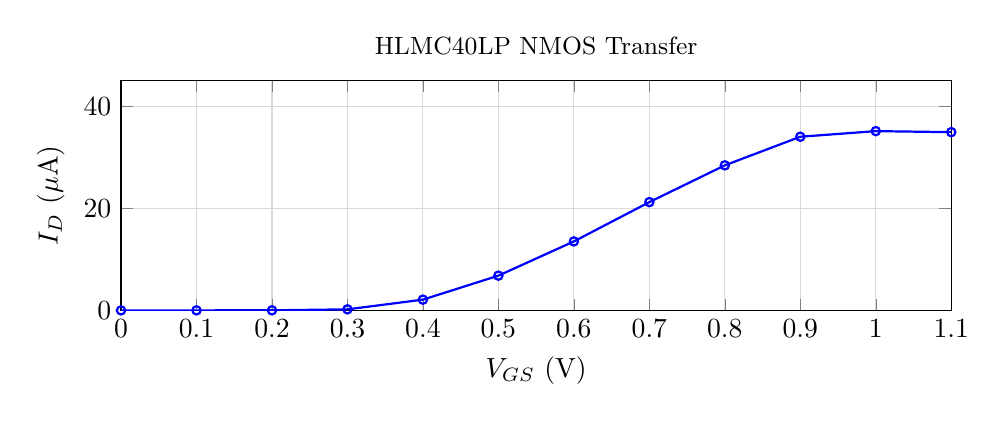
\begin{tikzpicture}
\begin{axis}[
    width=\columnwidth,
    height=4.5cm,
    xlabel={$V_{GS}$ (V)},
    ylabel={$I_D$ ($\mu$A)},
    xmin=0, xmax=1.1,
    ymin=0, ymax=45,
    grid=major,
    grid style={gray!30},
    title={\small HLMC40LP NMOS Transfer},
]
\addplot[blue, thick, mark=o, mark size=1.5pt] coordinates {
    (0.0, 0.0) (0.1, 0.0) (0.2, 0.01) (0.3, 0.2) (0.4, 2.1)
    (0.5, 6.8) (0.6, 13.5) (0.7, 21.2) (0.8, 28.4)
    (0.9, 34.0) (1.0, 35.1) (1.1, 34.9)
};
\end{axis}
\end{tikzpicture}
\caption{Transfer curve}
\end{subfigure}
\hfill
\begin{subfigure}[b]{0.48\columnwidth}
\centering
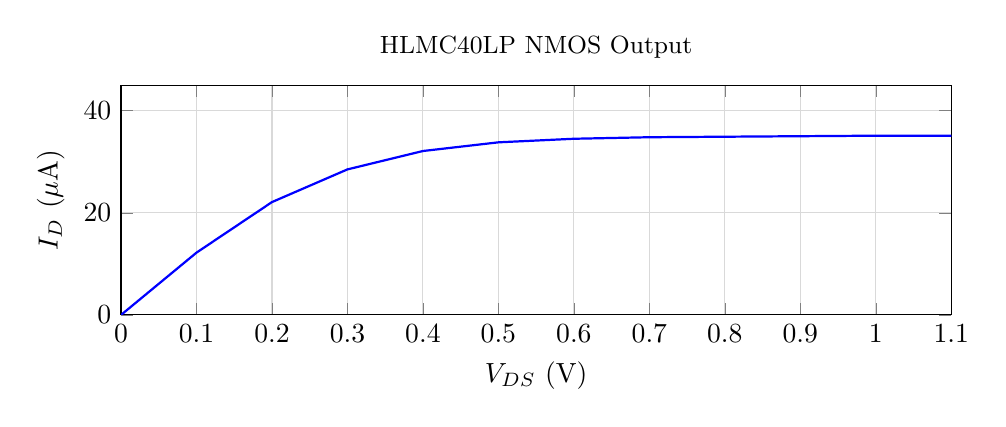
\begin{tikzpicture}
\begin{axis}[
    width=\columnwidth,
    height=4.5cm,
    xlabel={$V_{DS}$ (V)},
    ylabel={$I_D$ ($\mu$A)},
    xmin=0, xmax=1.1,
    ymin=0, ymax=45,
    grid=major,
    grid style={gray!30},
    title={\small HLMC40LP NMOS Output},
]
\addplot[blue, thick] coordinates {
    (0.0, 0.0) (0.1, 12.2) (0.2, 22.1) (0.3, 28.5) (0.4, 32.1)
    (0.5, 33.8) (0.6, 34.5) (0.7, 34.8) (0.8, 34.9)
    (0.9, 35.0) (1.0, 35.1) (1.1, 35.1)
};
\end{axis}
\end{tikzpicture}
\caption{Output family}
\end{subfigure}
\caption{HLMC40LP verification plots in the appendix.}
\label{fig:hlmc40lp_appendix}
\end{figure}

\begin{figure}[!t]
\centering
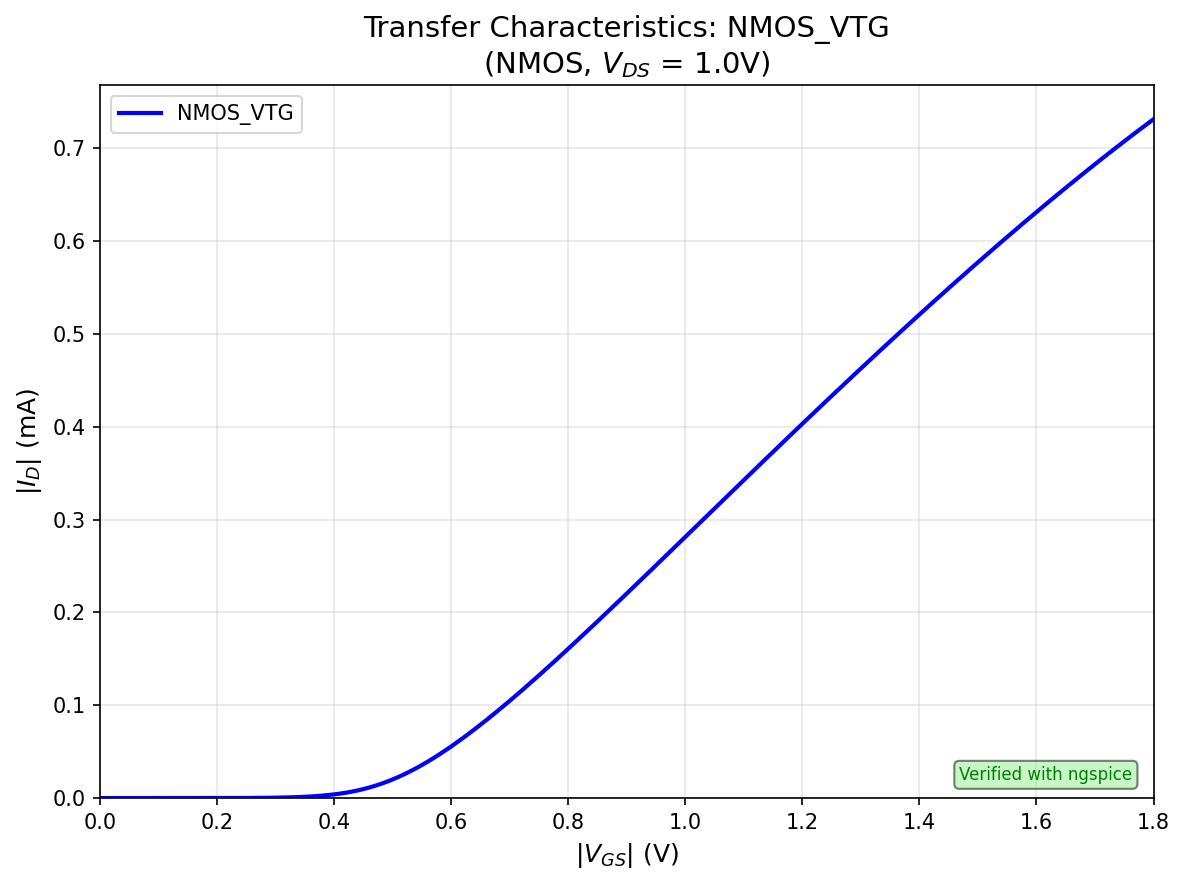
\includegraphics[width=0.47\columnwidth]{../output/freepdk45_hspice-ngspice/plots/NMOS_VTG_idvgs.png}
\hfill
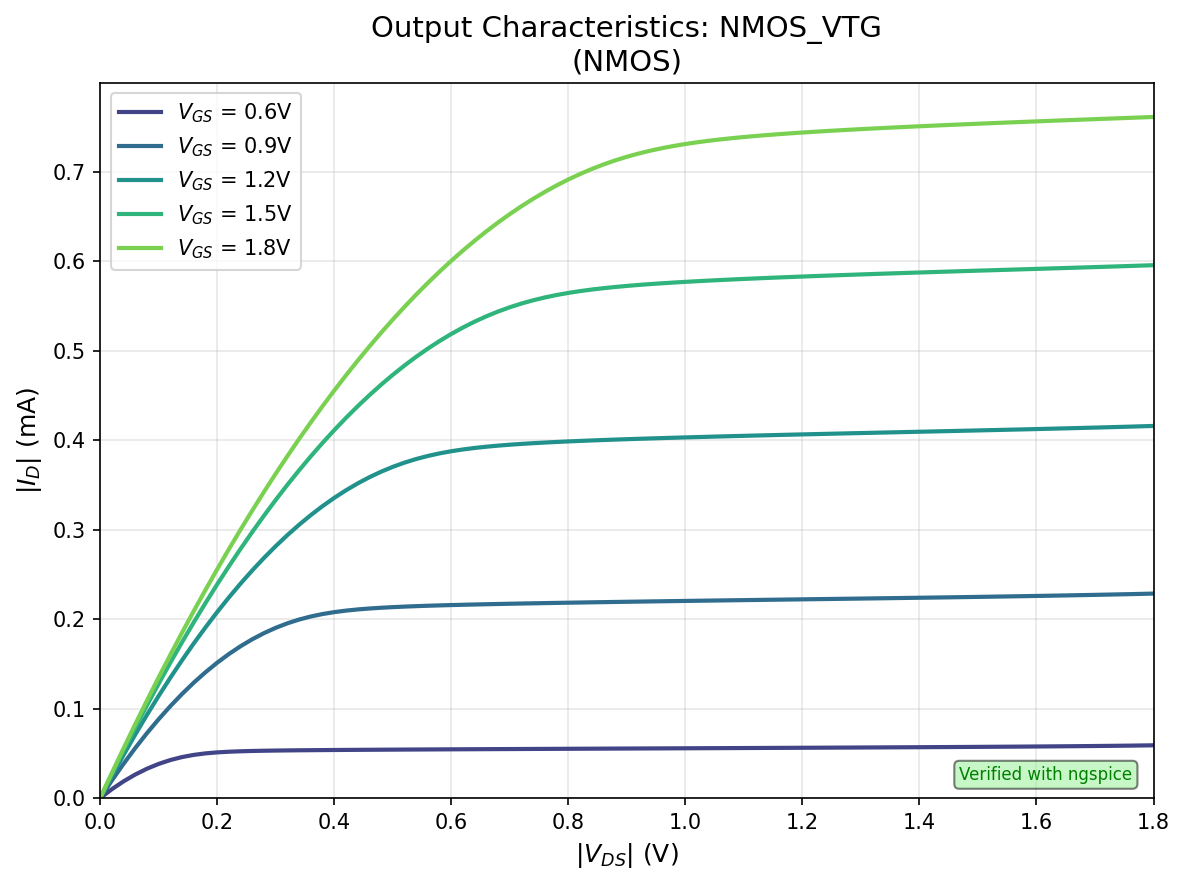
\includegraphics[width=0.47\columnwidth]{../output/freepdk45_hspice-ngspice/plots/NMOS_VTG_idvds.png}
\caption{FreePDK45 verification plots used in the current clean rerun.}
\label{fig:freepdk45_appendix}
\end{figure}

\begin{figure}[!t]
\centering
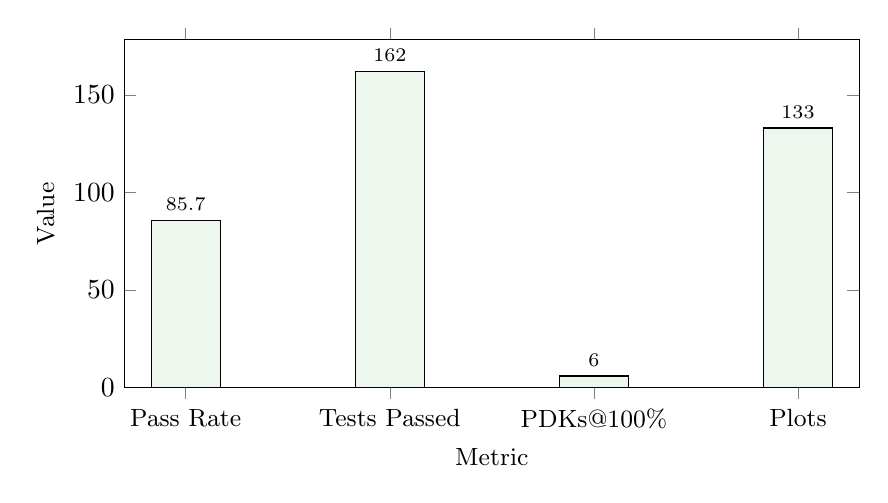
\begin{tikzpicture}
\begin{axis}[
    width=0.9\columnwidth,
    height=6cm,
    ybar,
    bar width=25pt,
    xlabel={Metric},
    ylabel={Value},
    ymin=0,
    xtick=data,
    symbolic x coords={Pass Rate, Tests Passed, PDKs@100\%, Plots},
    x tick label style={font=\small},
    ylabel style={font=\small},
    xlabel style={font=\small},
    nodes near coords,
    nodes near coords style={font=\scriptsize, above},
]
\addplot[fill=lightgreen!80] coordinates {
    (Pass Rate, 85.7)
    (Tests Passed, 162)
    (PDKs@100\%, 6)
    (Plots, 133)
};
\end{axis}
\end{tikzpicture}
\caption{ModelIR v4 verification achievements from the development-stage evaluation.}
\label{fig:overall_improvement_appendix}
\end{figure}

\begin{table}[!t]
\caption{Distribution of Pattern Matches in the Evaluation Corpus}
\label{tab:pattern_distribution_appendix}
\centering
\renewcommand{\arraystretch}{1.15}
\begin{tabular}{@{}lc@{}}
\toprule
\textbf{Pattern Class} & \textbf{Share} \\
\midrule
Scaling (\texttt{*\_eff}) & 32\% \\
Delta (\texttt{d*}, \texttt{del*}) & 28\% \\
Critical BSIM4 & 18\% \\
Device-specific & 15\% \\
Other / Default 0 & 7\% \\
\bottomrule
\end{tabular}
\end{table}

%==============================================================================
\balance
\bibliographystyle{plain}
\begin{thebibliography}{99}

\bibitem{spice70}
L. W. Nagel and D. O. Pederson, ``SPICE (Simulation Program with Integrated Circuit Emphasis),''
\textit{Univ. California, Berkeley}, Tech. Rep., 1973.

\bibitem{spice_reference}
K. Kundert, \textit{The Designer's Guide to SPICE and Spectre}.
Kluwer Academic, 1995.

\bibitem{ngspice}
H. Vogt, ``ngspice---Open Source SPICE Circuit Simulator,'' 
\url{https://ngspice.sourceforge.io/}, accessed Feb. 2026.

\bibitem{spectre}
Cadence Design Systems, ``Spectre Circuit Simulator Reference,''
Version 21.1, 2021.

\bibitem{hspice}
Synopsys Inc., ``HSPICE User Guide: Simulation and Analysis,''
Version U-2023.03, 2023.

\bibitem{hspice2}
M. Sievers, \textit{HSPICE User's Manual}, Synopsys Inc., 2015.

\bibitem{circuit_simulation}
R. A. Rohrer and H. Nosrati, ``Lumped-element representation of distributed circuits,''
\textit{IEEE Trans. Circuits Syst.}, vol. CAS-24, no. 2, pp. 49--59, Feb. 1977.

\bibitem{mna_analysis}
C. W. Ho, A. E. Ruehli, and P. A. Brennan, ``The modified nodal approach to network analysis,''
\textit{IEEE Trans. Circuits Syst.}, vol. CAS-22, no. 6, pp. 504--509, June 1975.

\bibitem{bsim4}
Y. Cheng et al., \textit{MOSFET Modeling \& BSIM3 User's Guide}. 
Springer, 1999.

\bibitem{bsim_history}
C. Hu, ``BSIM Model for Circuit Simulation,'' 
\textit{IEEE Circuits Devices Mag.}, vol. 12, no. 5, pp. 21--26, 1996.

\bibitem{bsim3_ref}
Y. Cheng, C. Hu, P. Vande Walle, and M. Chan, ``BSIM3 physical behavior and performance improvements,''
in \textit{Proc. Int. Conf. Modeling Simulation Microsyst.}, 1998.

\bibitem{bsim_coremodel}
Y. S. Chauhan et al., ``BSIM-CMG 110.0.0: A Scalable Compact Model for Multi-Gate MOSFETs,''
\textit{IEEE Trans. Electron Devices}, vol. 60, no. 10, pp. 3408--3422, Oct. 2013.

\bibitem{bsim_cmg}
Y. S. Chauhan et al., ``BSIM-CMG 110.0.0 Multi-Gate MOSFET Compact Model,''
Tech. Rep., UC Berkeley, 2020.

\bibitem{bsim_soi}
Y. S. Chauhan et al., ``BSIM-SOI Model Implementation,''
\textit{IEEE J. Electron Devices Soc.}, vol. 1, no. 9, pp. 295--305, 2013.

\bibitem{pdk_methodology}
R. J. Baker, \textit{CMOS: Circuit Design, Layout, and Simulation}, 3rd ed.
Wiley-IEEE Press, 2010.

\bibitem{characterization_methods}
C. McAndrew et al., ``Statistical modeling for IC applications,''
in \textit{Proc. Int. Conf. Simulation Semicond. Processes Devices (SISPAD)}, 2003.

\bibitem{corner_analysis}
J. F. Smith, ``Corner analysis for statistical design,''
\textit{Proc. Design Autom. Conf. (DAC)}, pp. 1--6, 2005.

\bibitem{monte_carlo}
R. H. Hocevar, ``Circuit-level modeling of process variability,''
\textit{IEEE Trans. Semicond. Manuf.}, vol. 12, no. 1, pp. 63--76, Feb. 1999.

\bibitem{openpdk}
T. Edwards et al., ``The Open PDK Project,''
\url{https://github.com/google/open-pdk}, 2023.

\bibitem{skywater}
Google and SkyWater Technology, ``SkyWater SKY130 PDK,''
\url{https://github.com/google/skywater-pdk}, 2023.

\bibitem{gf180}
GlobalFoundries, ``GF180MCU Open Source PDK,''
\url{https://github.com/google/gf180mcu-pdk}, 2023.

\bibitem{compiler_design}
A. V. Aho, M. S. Lam, R. Sethi, and J. D. Ullman, \textit{Compilers: Principles, Techniques, and Tools}, 
2nd ed. Boston, MA: Addison-Wesley, 2006.

\bibitem{lex_yacc}
M. E. Lesk and E. Schmidt, ``Lex---A Lexical Analyzer Generator,''
\textit{Comput. Sci. Tech. Rep.}, AT\&T Bell Labs, 1975.

\bibitem{design_patterns}
E. Gamma, R. Helm, R. Johnson, and J. Vlissides, \textit{Design Patterns: Elements of Reusable Object-Oriented Software}.
Boston, MA: Addison-Wesley, 1994.

\bibitem{asap7}
L. T. Clark et al., ``ASAP7: A 7-nm FinFET Predictive Process Design Kit,''
\textit{Microelectron. J.}, vol. 53, pp. 105--115, 2016.

\bibitem{virtuoso}
Cadence Design Systems, ``Virtuoso ADE Product Suite,''
\url{https://www.cadence.com/}, 2024.

\bibitem{netlist}
C. D. Motchenbacher and J. A. Connelly, \textit{Low-Noise Electronic System Design},
Wiley-Interscience, 1993.

\end{thebibliography}

\end{document}
